\documentclass[a4paper]{article}

\usepackage{numprint}
\usepackage{nameref}
\usepackage{float}
\usepackage{url}
\usepackage{graphicx}	% For figure environment
\usepackage{epstopdf}
\usepackage[center]{subfigure}
\usepackage{amssymb}	% For mathematical figures like \mathbb{R}
\usepackage{amsmath}
\usepackage{framed}
\usepackage{tikz}
\usetikzlibrary{mindmap,trees}
\usepackage{pdflscape}
\usepackage[a4paper]{geometry}
\usepackage{subfiles}
\usepackage{listings}
\usepackage{color}
\usepackage{parskip}

\definecolor{dkgreen}{rgb}{0,0.6,0}
\definecolor{gray}{rgb}{0.5,0.5,0.5}
\usepackage{array}
\usepackage{booktabs}% http://ctan.org/pkg/booktabs
\usepackage{xparse}% http://ctan.org/pkg/xparse
% Rotation: \rot[<angle>][<width>]{<stuff>}
\NewDocumentCommand{\rot}{O{45} O{1em} m}{\makebox[#2][l]{\rotatebox{#1}{#3}}}%
\definecolor{mauve}{rgb}{0.58,0,0.82}

\lstset{frame=tb,
  language=Java,
  aboveskip=3mm,
  belowskip=3mm,
  showstringspaces=false,
  columns=flexible,
  basicstyle={\small\ttfamily},
  numbers=none,
  numberstyle=\tiny\color{gray},
  keywordstyle=\color{blue},
  commentstyle=\color{dkgreen},
  stringstyle=\color{mauve},
  breaklines=true,
  breakatwhitespace=true
  tabsize=3
}


\title{Advanced Systems Lab - Milestone II} 
\author{Lukas Elmer (elmerl@ethz.ch)} 
\date{\today} 


\begin{document}

\maketitle

\pagebreak

\tableofcontents

\pagebreak

\begin{abstract}

This document is the follow up document of Advanced Systems Lab - Milestone I \cite{milestone1} and describes an analytical queueing model of the system which was built using the operational laws. Using this model, the performance characteristics of the model are derived and compared to the measurements of Milestone I \cite{milestone1}. Furthermore it is analysed where the data matches the model and where it does not.

\end{abstract}

\pagebreak

\section{Introduction}

\subsection{Assumptions}

First, we have to make some assumptions, so we can apply the operational laws. They are as follows:

\begin{itemize}
\item First, we assume that the system is \textbf{homogeneous}. This means that the behaviour of jobs or resources doesn't depend on the global state of the system.
\item The system is \textbf{job flow balanced}. This means that the same amount of requests are completed by the system as arrive at the system. In practice, this means that a) no requests are "lost" and b) no requests take infinite amount of time.
\item This implicitly means that no jobs are destroyed or created within the system. This is also called \textbf{conservation of work}.
\end{itemize}

However, these assumptions may easily be violated. Examples:\\

The first assumption is not entirely true for the system, because the computational capacity of the Amazon machines may very well depend on the workload of the physical server, because other people might use the same server/network at the same time. Another possibility which would influence the system would be the operating system, which may run some background jobs. Another example may be the garbage collector of the JVM, which may interfere. Lastly, we consider some SSH connection to the server, which also influences the performance. However, we assume that all those interferences are minor and don't influence the system at great scale.\\

Even tough there are unit tests which support the stability of the system, it is possible that the system may contain a bug, which in the worst case could destroy a job. Therefore, the third assumption (and therefore also the second one) can be violated. However, this should not happen, and there are also system logs where most of these possible errors would be logged.\\

\subsection{Data Sources}

This document extends the document of milestone I\cite{milestone1}. Especially the following test runs are used in this analysis:

\begin{itemize}
\item Microbenchmarks (conducted during last milestone\cite{milestone1})
\item 2 hour test (conducted during last milestone\cite{milestone1})
\item Scaleout experiments (conducted during this milestone, see below)
\end{itemize}

\subsubsection{Scaleout Experiments}

Some additional scaleout experiments were conducted. They were executed with 4 middlewares distributed on 2 virtual machines. For the client and middleware instances, Amazon instances of the type m1.small was used, and for the database the type m1.medium was used.\\
\noindent Then, the number of clients was scaled from in steps of 15 from 15-60, and in steps of 30 from 60-300.


\pagebreak

\section{Components}

In the analysis, the focus of the system is on the middleware. Additionally, the database is modelled as a queue, but no further internals of the database are considered.\\

\begin{figure}[H]
	\begin{center}
    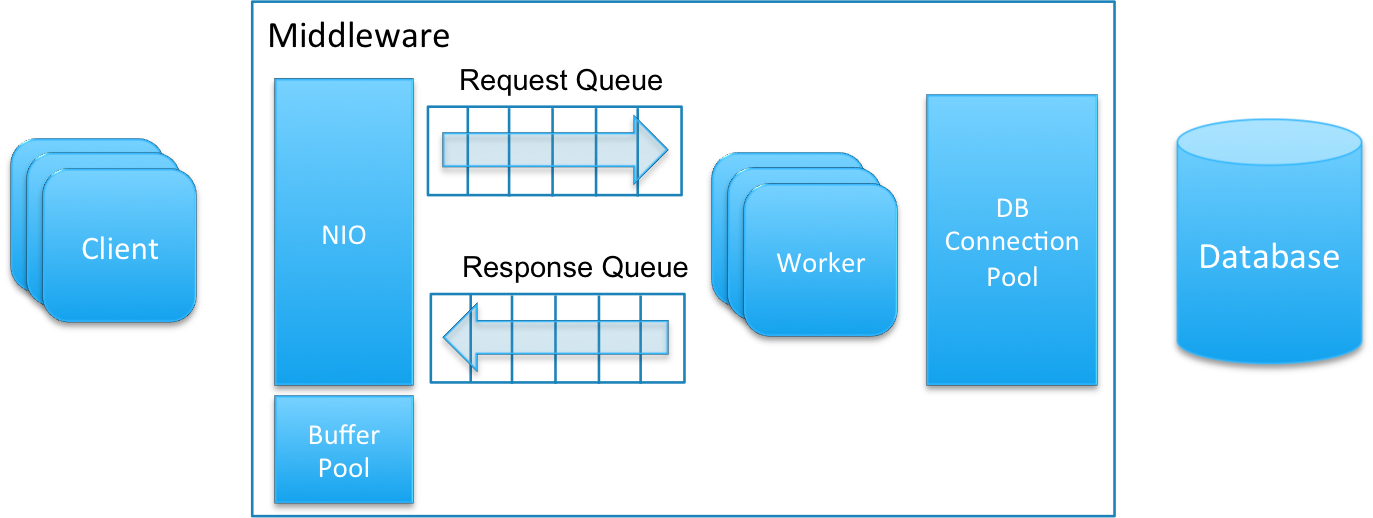
\includegraphics[scale=0.6]{../drawings/broker-threading.png}
  \end{center}
  \caption{Middleware's main Components}
  \label{fig:middleware-threading}
\end{figure}

Figure \ref{fig:middleware-threading} shows a overview of the systems components. The most important parts of the analytical models are:

\begin{itemize}
\item The middleware (multiple instances)
	\begin{itemize}
	\item NIO (network input and output, single queue)
	\item Request queue (when the requests are waiting for workers)
	\end{itemize}
\item The database (modelled as a single queue)
\end{itemize}

Because the clients wait for the current message to be answered before sending the next message, the system is modelled as a \textbf{closed system}. If messages fail to be processed by the middleware, the client implements a backoff time, so the system doesn't get overloaded.

\section{Performance Characteristics}

As described in the textbook \cite{Raj} in section 30.1, a queuing system can be specified by six parameters. Therefore we use the Kendall notation in the form A/S/m/B/K/SD, where the letters correspond to the six parameters listed on page 507-509 in the textbook\cite{Raj}. Unless specified otherwise, when A/S/m is written, then this corresponds to a A/S/m/$\infty$/$\infty$/FCFS queue, where FCFS means First Come First Serve\footnote{https://en.wikipedia.org/wiki/First-come,\_first-served}.

\subsection{A: Arrival Process}

Even tough the clients send in a certain deterministic interval, because of the network and the operating system there is a delay until the requests arrive in the queuing system. We assume that this delay is exponentially distributed. Thus, A is the Markovian M.

\subsection{S: Service Time Distribution}

The service time distribution also is assumed to be distributed exponentially. We also know that the service time is memoryless - i.e. it does not matter what request happened before the current request. This can be assumed because there is no caching implemented.

\subsection{m: Number of Servers}

The number of servers is the amount of middlewares running.

\subsection{B: System Capacity}

The system capacity is defined by those who are waiting for service and those who receive service.  This is dependent on how many requests a middleware can accept. Because there are always less clients connected to a middleware then connections to the NIO part of the middlware can be established, the system capacity will be the same as the population size.\\

Unless otherwise specified, 

\subsection{K: Population Size}

The population size is defined by the amount of clients issuing requests to the middleware.

\subsection{SD: Service Discipline}

In general, the service discipline is First Come, First Served (FCFS). However, because there are limited CPU's on the middleware, and CPU's usually use Round Robin (RR), this may have to be considered in the analysis.


\pagebreak

\section{Model}

\subsection{General Model}

The following queueing model network was created based on the understanding of the closed system as shown in figure \ref{fig:general-queueing-network}.

\begin{figure}[H]
	\begin{center}
    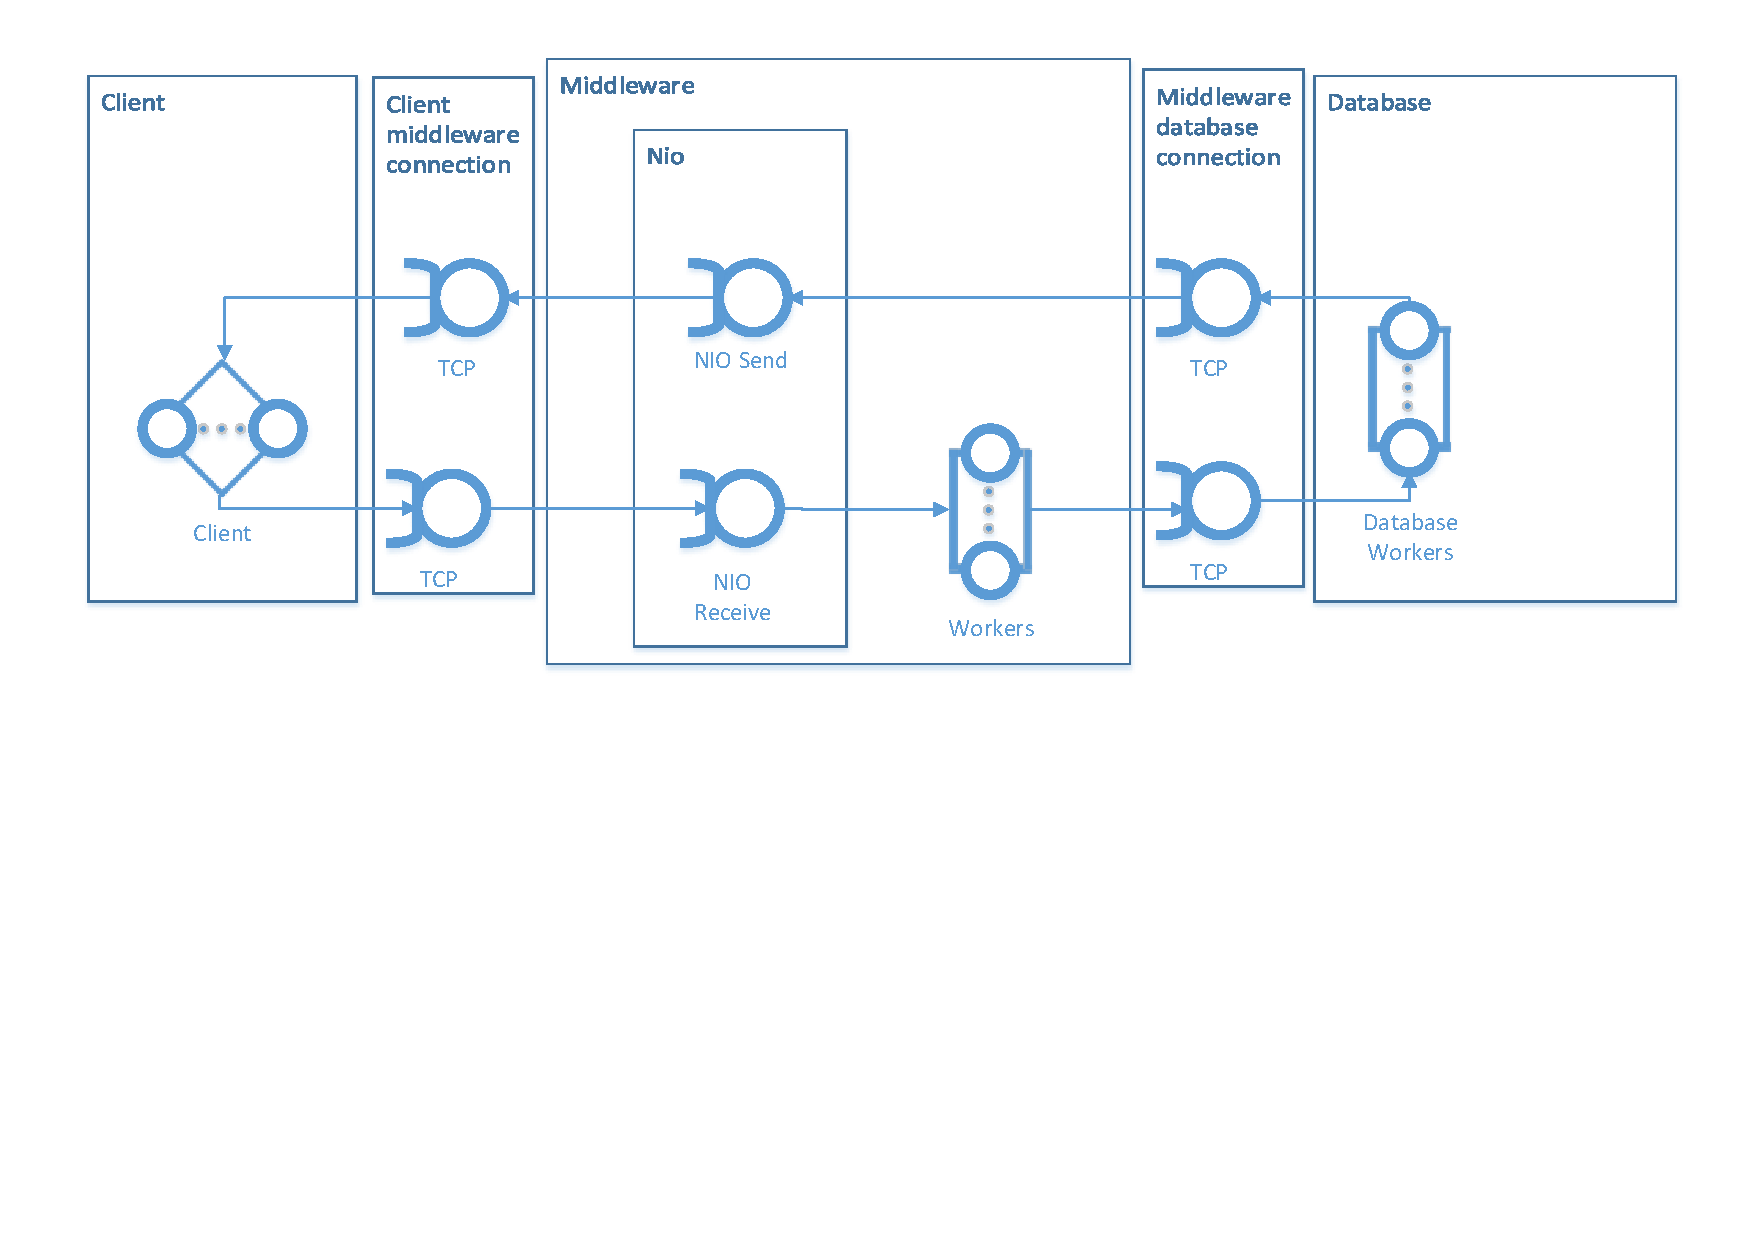
\includegraphics[scale=0.6, trim = 15mm 94mm 12mm 10mm, clip]{../drawings-ms2le/general-queueing-network.pdf}
  \end{center}
  \caption{general queueing network}
  \label{fig:general-queueing-network}
\end{figure}


\subsection{Simplified Model}

Initially the TCP connections are modelled as a separate System. To be precise, these TCP connections would influence one another. In the simplified model, those TCP connections act as separate queues. Additionally, the NIO part of the middleware is included in the TCP connection queue. This is a good idea because the NIO thread and the network are strongly linked and the NIO processing is very fast.\\

Next, the model was further simplified by separating the NIO component into two separate queues. In the real system however, similar to the TCP connection, there is only one NIO thread.\\

Furthermore, the TCP network connection between the middleware and the database is separated. In the real system, this would be the same connection.\\

To further simplify the model, the TCP connections are modeled as delay centers instead of queues. This should be ok, because the network connection utilization is not at it's limit during the test runs.\\

Those simplifications then lead to the simplified queueing network as shown in figure \ref{fig:simplified-queueing-network}. Note that the TCP connections are still drawn as queues, but they are modeled as delay centers instead.\\


\begin{figure}[H]
	\begin{center}
    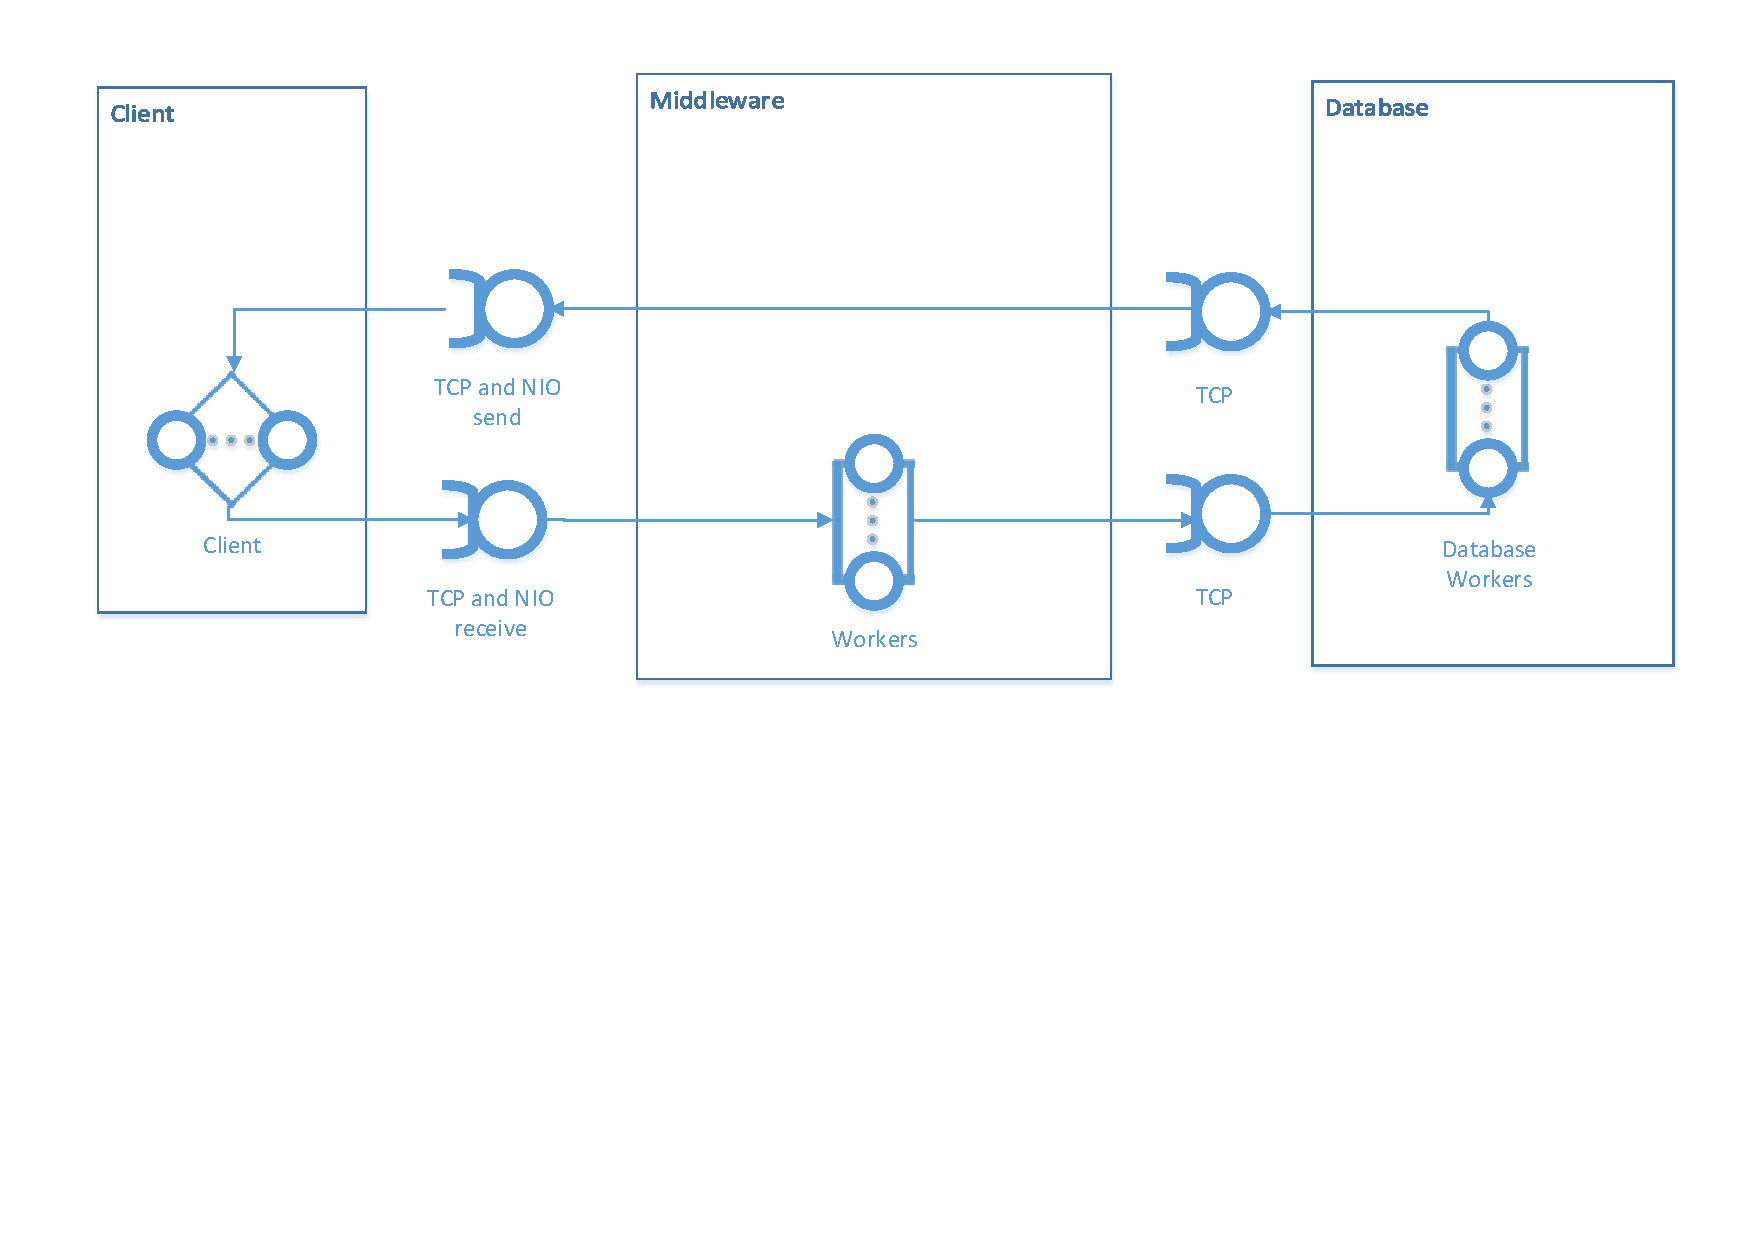
\includegraphics[scale=0.6, trim = 15mm 94mm 12mm 10mm, clip]{../drawings-ms2le/simplified-queueing-network.pdf}
  \end{center}
  \caption{simplified queueing network}
  \label{fig:simplified-queueing-network}
\end{figure}

\subsection{Service Centers}

\subsubsection{Client: M/M/$\infty$/$\infty$/$\infty$/FCFS}

The clients do simple operations (send and receive messages) and don't do any computation. The think time (\textbf{Z}) of the client doesn't depend on the client count and thus correspond to the sleep time between requests.\\

The think time of the clients is 10ms.\\

For the scaleout test, the number of clients was scaled from 15, 30, 45, 60.

\subsubsection{TCP and NIO receive / send: M/M/$\infty$/$\infty$/$\infty$/FCFS}

The TCP and NIO receive / send contains many things like the network card, the time it takes to physically transport and rout the signal to the corresponding receiver, the OS buffer, and the JVM network buffer. It was decided to also add the NIO thread to this queue, because it acts like the OS buffer or the JVM network buffer.\\

According to the Java specification, the buffer of the TCP connection is 50, and thus the queue should be modeled as M/M/$\infty$/50/$\infty$/FCFS. However, to simplify the model, it is modeled as M/M/$\infty$/$\infty$/$\infty$/FCFS.\\

The queue is modelled as a fixed capacity service center with and unbound queue size. Because only one network connection and one NIO thread is used, the service node count is 1. So it is modelled as M/M/$\infty$/$\infty$/$\infty$/FCFS queue.\\

In the following analysis, the "TCP and NIO receive" and the "TCP" are merged together as TCP.\\

Another thing that could have been modelled would have been the separation of sending and receiving messages. For this, the database would be split up into two parts, one for sending and one for receiving respectively. However, to keep the model simple, this hasn't been done.\\


\subsubsection{TCP M/M/$\infty$/$\infty$/$\infty$/FCFS}

This is the same as \textbf{TCP and NIO receive} without the NIO. Therefore it is also modelled as a fixed capacity service center with unbound queue size and a node count of 1.\\

As measured in the milestone I\cite{milestone1}, the mean service time of the TCP connection is 2.644ms for sending and 2.590ms for receiving messges. For this analysis, the mean of 2.617ms is assumed to simplify the analysis.\\

In the following analysis, the "TCP and NIO receive" and the "TCP" are merged together as TCP.


\subsubsection{Workers (Middleware): 80 * M/M/1/$\infty$/$\infty$/FCFS}

There are several worker threads in the system. These worker threads are modelled as a M/M/x queue, where x corresponds to the number of worker threads per middleware. The workers obviously are load dependent. The queue size is 100, as it corresponds to the queue size of the queue from which the worker threads can get the requests which have to be processed.\\

Additionally, the middlewares can be scaled. The clients are evenly distributed between the middlewares, and so are the requests sent by the clients. Therefore, the model is simplified further as follows: for every additional middleware, the workers are merged into one big worker pool across all middlewares. Therefore, the middleware queues are modelled as (n * x) * M/M/1/$\infty$/$\infty$/FCFS queues, where n corresponds to the amount of middlewares and x corresponds to the number of worker threads per middleware.\\

For the scaleout test, 4 middlewares were used, each with 20 workerthreads. This gives a total of $4*20 = 80$. The visit count for the middleware is therefore 1/80, because one messages passes through exactly one middleware worker.\\

The service time of the middleware is calculated as follows:
$$Total service time - DB service time - 4 * TCP service time$$
As estimated in the milestone I\cite{milestone1}, for sending the service time is 0.042ms and for receiving it is 0.043ms. For the analysis, a service time of 0.042ms is used.\\


\subsubsection{Database M/M/8/$\infty$/$\infty$/FCFS}

As stated in the requirements, there must be only one database. However there is never a global table lock and there are multiple ECU's (EC2 Compute Unit\footnote{https://aws.amazon.com/en/ec2/faqs/\#What\_is\_an\_EC2\_Compute\_Unit\_and\_why\_did\_you\_introduce\_it})  available. Furthermore it's unknown how the hardware of the Amazon medium instance is exactly built, but it can be considered that it takes advantage of advanced technology like the locality effect, caching, fail-safe and performance optimized hardware. Unfortunately in one hand, fortunately in the other hand, details about the hardware which the system runs on is unknown. Further information can be found on the amazon website\footnote{https://aws.amazon.com/en/ec2/instance-types/}.\\

Even tough there are 2 ECU's: because there is one vCPU for the medium instance, the node count was first set to 1. Unfortunately this yielded bad results. Therefore, multiple values for the node count were tested. The best results were achieved with a node count of 8. One reason to explain this may be that the database implements bulk IO operations and stores the corresponding pages in the cache. Also, the vCPU instance implements hyperthreading, so more vCPU power is available than only one vCPU.\\

The service center is modelled as load dependent for obvious reasons.\\

The service time is 4.016ms for sending and 6.196ms for receiving messages, as measured in the microbenchmarks. For this analysis, the mean of 5106ms was used first. Unfortunately, because sending a message is faster then receiving a message, there are more messages sent then received. Therefore the service time for the database had to be adjusted to 4.506ms.\\



\pagebreak

\section{Mean Value Analysis}

The mean value analysis is performed as described in the book used in this course \cite[Box 34.3, Box 35.1, Box 36.1]{Raj}. Here, the values of the microbenchmarks of milestone I\cite{milestone1} are used. Furthermore, the mean value analysis is also based on the scaleout experiments conducted during this milestone.\\


%To calculate the mean arrival time and the mean service rate, the scaleout experiment with 60 clients was used. This gives a mean arrival rate ($\lambda$) 178.885 messages per second. The mean service time for this test was 32.99374762ms, and there are 80 workers, which gives a mean service rate of 1 / 32.99374762ms / 80 workers = 0.37885966 requests/s/worker and 30.30877278 requests/s in total. \\

Here, all values from above and from milestone I\cite{milestone1} are listed. They are used as input for the mean value analysis.\\

The number of clients varies from 15-300\footnote{from 15-60 in steps of 15, from 60-300 in steps of 30}.\\

\begin{table}[h!]
\begin{center}
\begin{tabular}{|l|l|r|}
\hline
\textbf{Variable} & \textbf{Description} & \textbf{Value} \\ \hline
$N_{client}$ & \# clients & 15-300 \\ \hline
Z & client think time & 10ms \\ \hline
$N_{middleware}$ & \# middleware workers & 80 \\ \hline
$S_{middleware}$ & middleware service time & 0.042ms \\ \hline
$V_{middleware}$ & middleware visit count & 1/80 \\ \hline
$N_{tcp}$ & \# TCP & 80 \\ \hline
$S_{tcp}$ & TCP service time & 2.617ms \\ \hline
$V_{tcp}$ & TCP visit count & 4 \\ \hline
$N_{db}$ & \# DB Workers & 8 \\ \hline
$S_{db}$ & DB service time & 5.106ms \\ \hline
$S_{db}$ & DB service time (fixed version) & 4.506ms \\ \hline
$V_{db}$ & DB visit count & 1 \\ \hline
\end{tabular}
\caption{MVA input variables}
\end{center}
\end{table}

To do the analysis, a Java program was written. It can be found in the code/mean\_value\_analysis directory.\\

\subsection{Results}

Here, in the figures \ref{fig:rt-total}, \ref{fig:tp-total}, \ref{fig:rt-total-fixed} and \ref{fig:tp-total-fixed}, the model and the measured data are compared.

\subsubsection{Interpretation}

The first analysis without the adjusted service time for the database yielded not so good results for the response time. The mean value analysis for the response time seems pretty well. However, there seemed to be a additional constant of about 50ms where the response time of the model didn't match. It clearly can be observed that the measured response time and the modelled response time diverge, see figure \ref{fig:rt-total}. Also, the measured throughput is clearly higher then the modelled throughput, see figure \ref{fig:tp-total}. For those reasons, the mean service time of the database was adjusted and the fixed model was generated.\\

The analysis of the fixed model yields decent results, especially for the response time, which can be seen in figure \ref{fig:rt-total-fixed}. The predicted values of the model are well in between the standard deviation of the measured datapoints.\\

The throughput model and the measured datapoints can be compared in figure \ref{fig:tp-total-fixed}. Unlike the response time, the throughput model seems to be less accurate then the response time model. This is somewhat strange because they are related with the formula $Throughput=\frac{Users}{ResponseTime + ThinkTime}$. This will be further discussed in section \ref{sec:measurement-analysis}.


\subsubsection{Possible Further Investigations}

As described in the simplified model description, the system could be modelled differently, by splitting up the database for sending and receiving into two separate parts. I think that this way, the model would be more accurate compared to the measured data. However, the trade-off between model complexity and best fit is always tricky, and I chose to stay with the slightly simplified model.


\begin{landscape}\begin{figure}[H]
	\begin{center}
    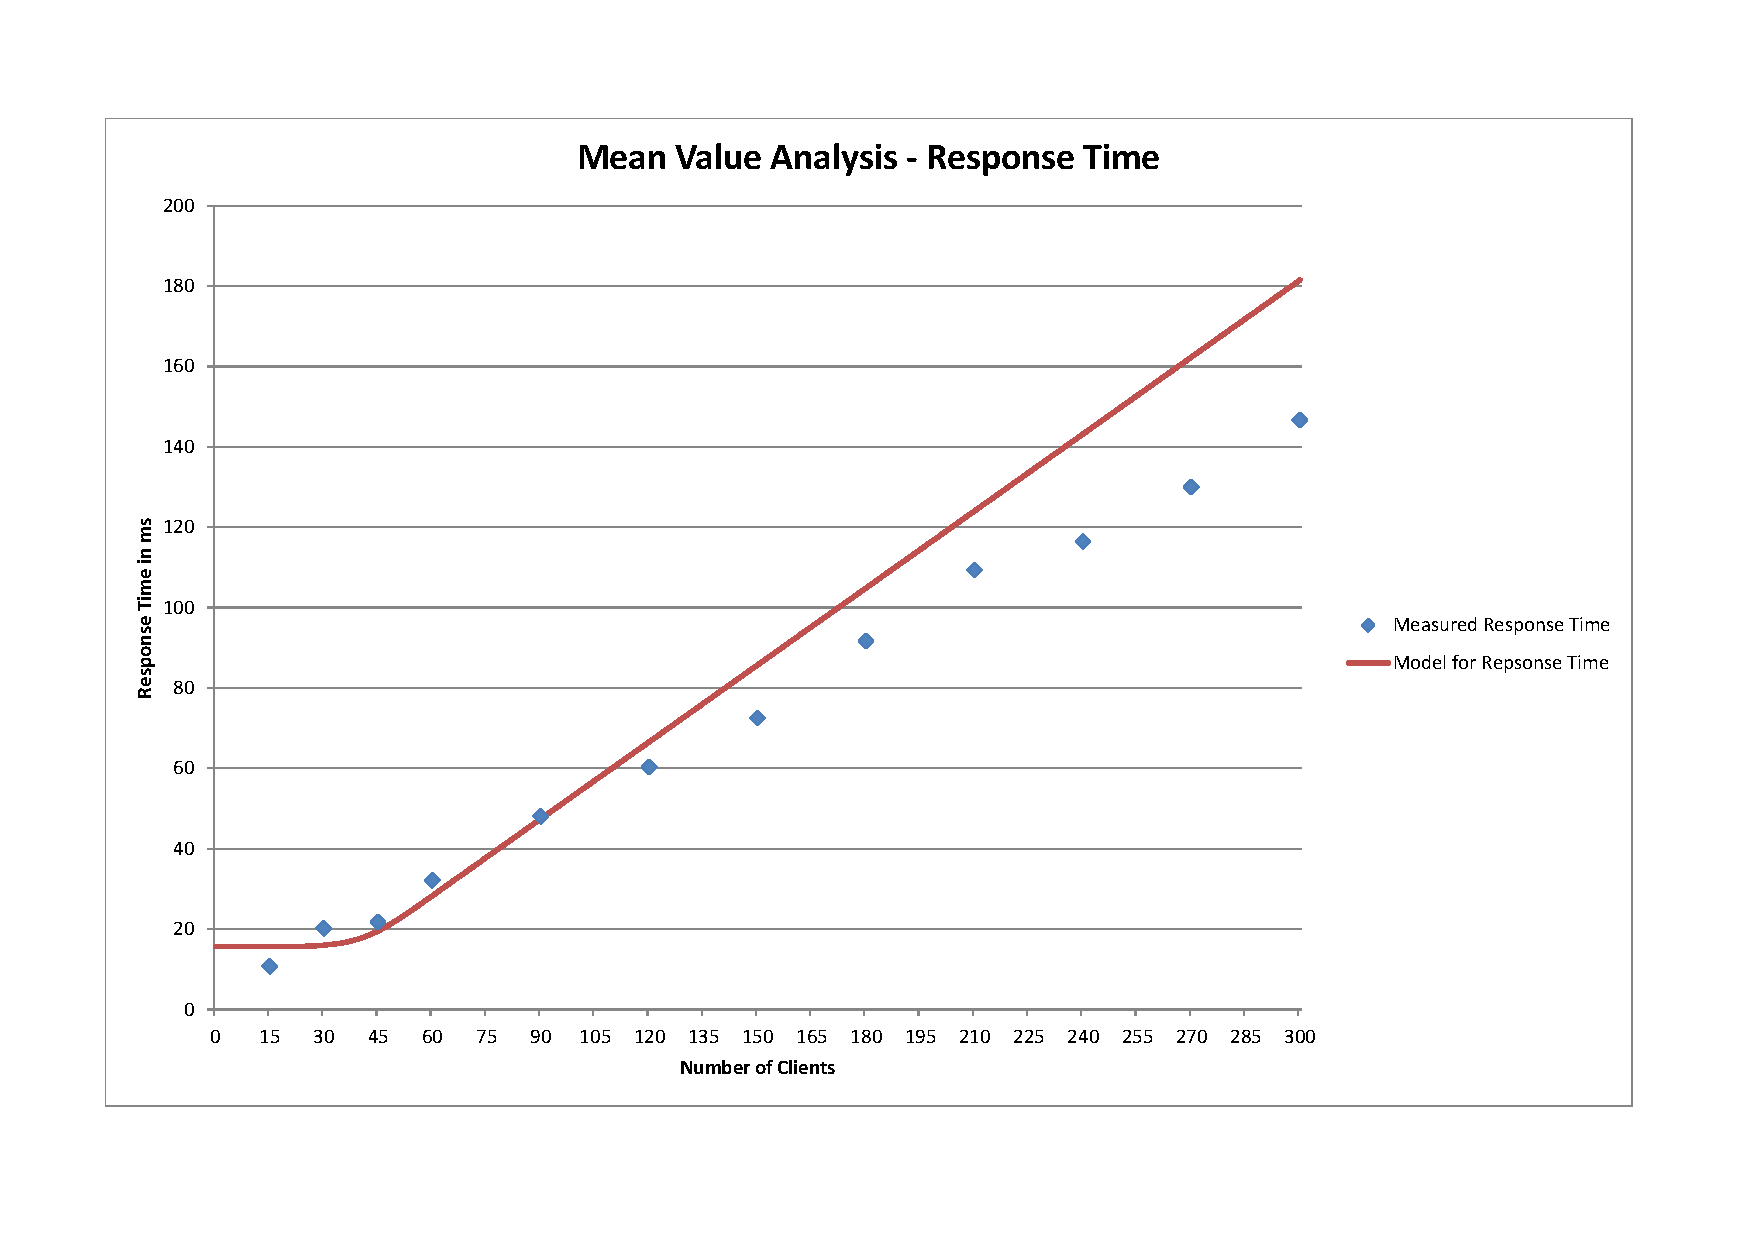
\includegraphics[scale=0.7, trim = 23mm 28mm 24mm 24mm, clip]{measurements_increase_load/rt_total.pdf}
  \end{center}
  \caption{mean value analysis, response time, with standard deviation}
  \label{fig:rt-total}
\end{figure}

\begin{figure}[H]
	\begin{center}
    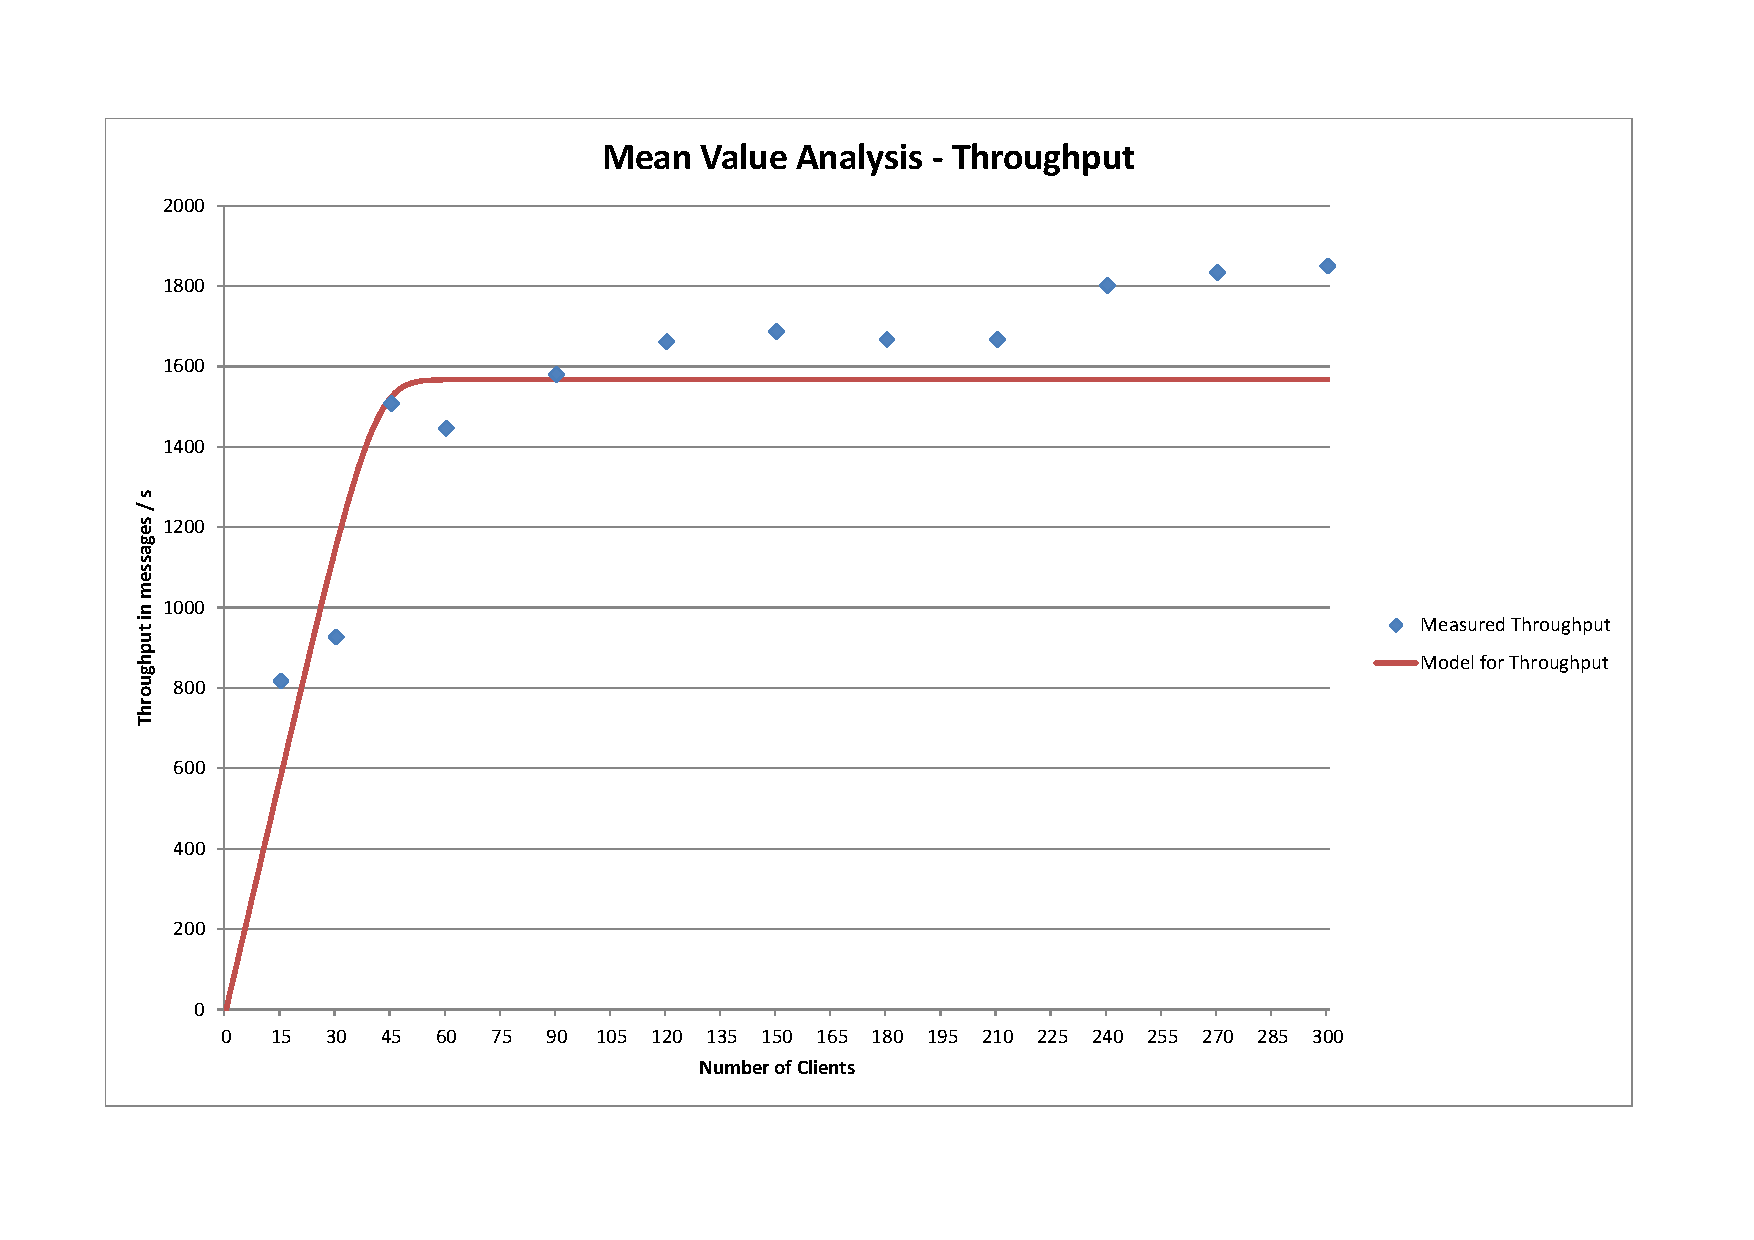
\includegraphics[scale=0.7, trim = 23mm 28mm 24mm 24mm, clip]{measurements_increase_load/tp_total.pdf}
  \end{center}
  \caption{mean value analysis, throughput}
  \label{fig:tp-total}
\end{figure}


\begin{figure}[H]
	\begin{center}
    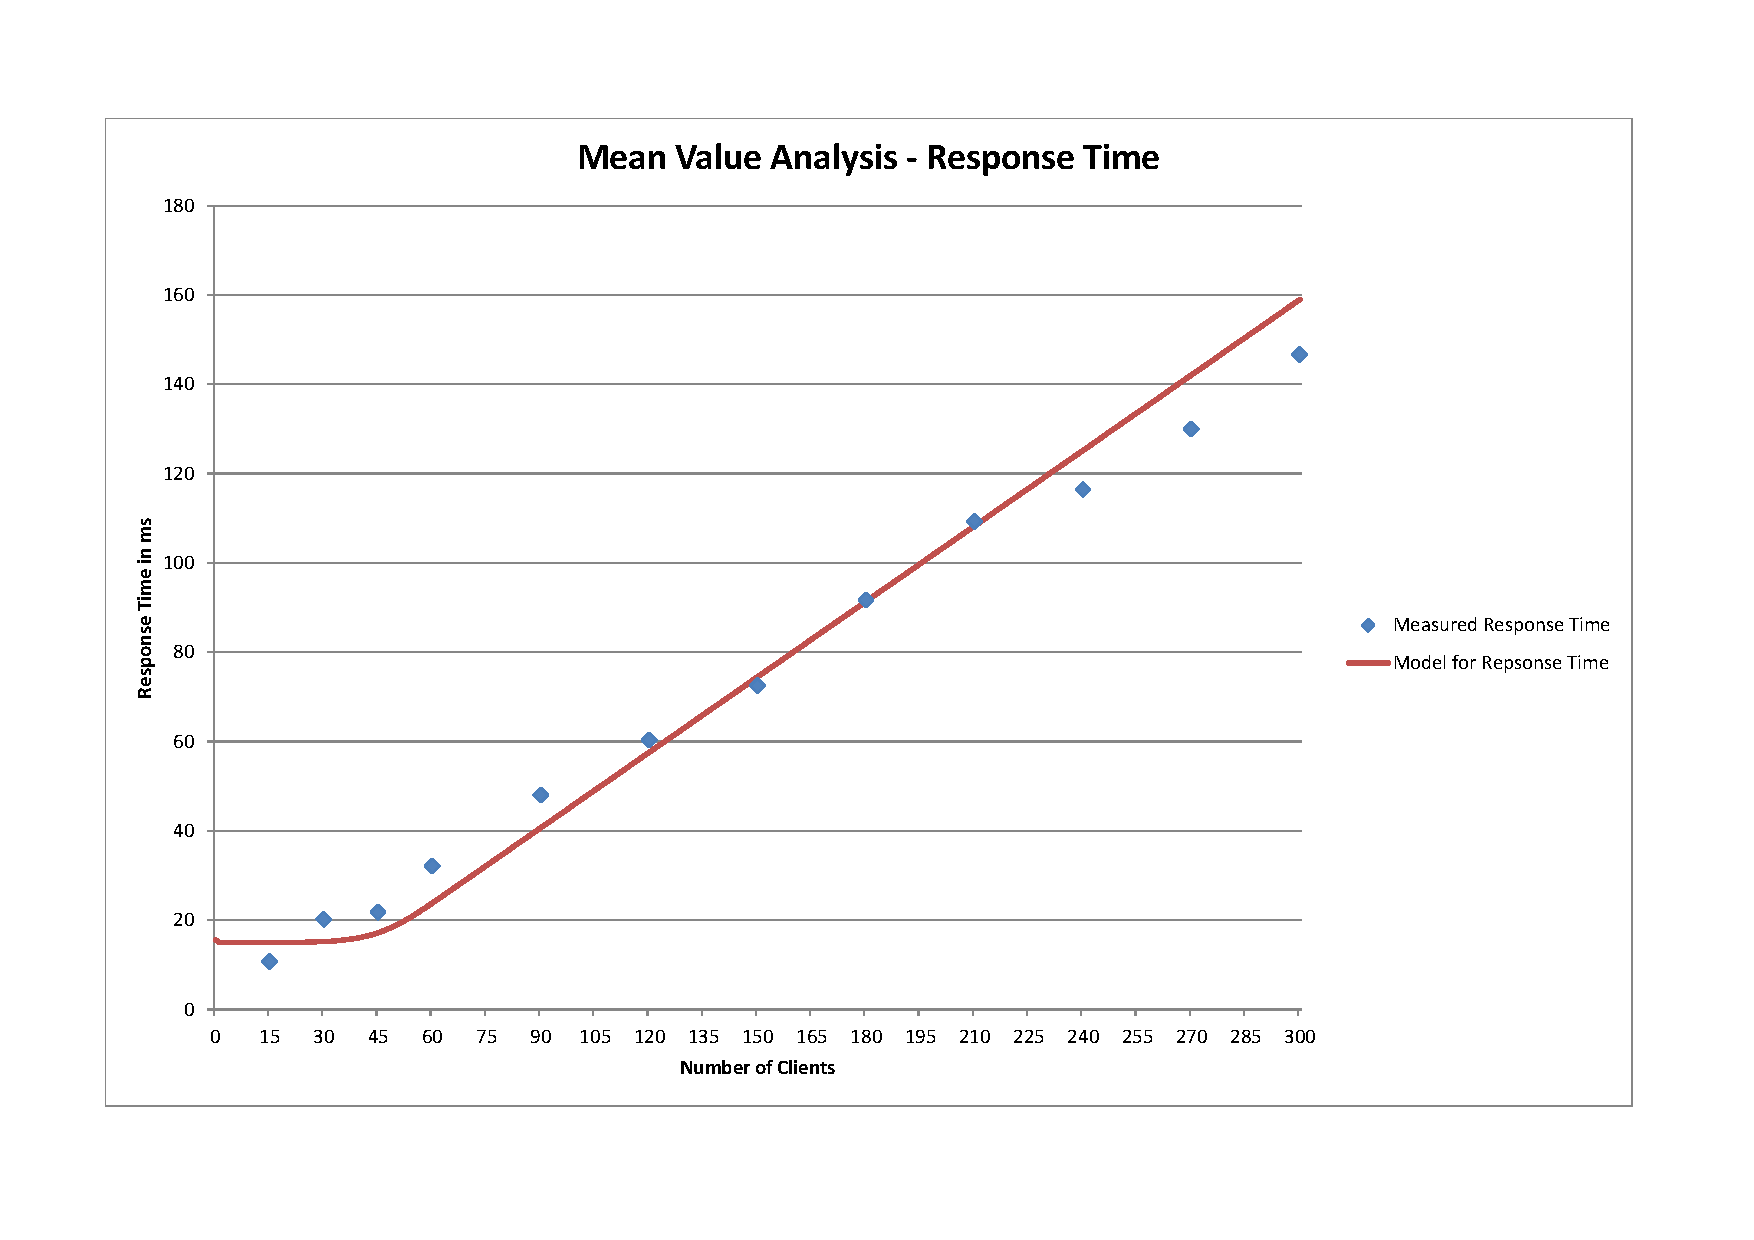
\includegraphics[scale=0.7, trim = 23mm 28mm 24mm 24mm, clip]{measurements_increase_load/rt_total_fixed.pdf}
  \end{center}
  \caption{mean value analysis, response time fixed, with standard deviation}
  \label{fig:rt-total-fixed}
\end{figure}

\begin{figure}[H]
	\begin{center}
    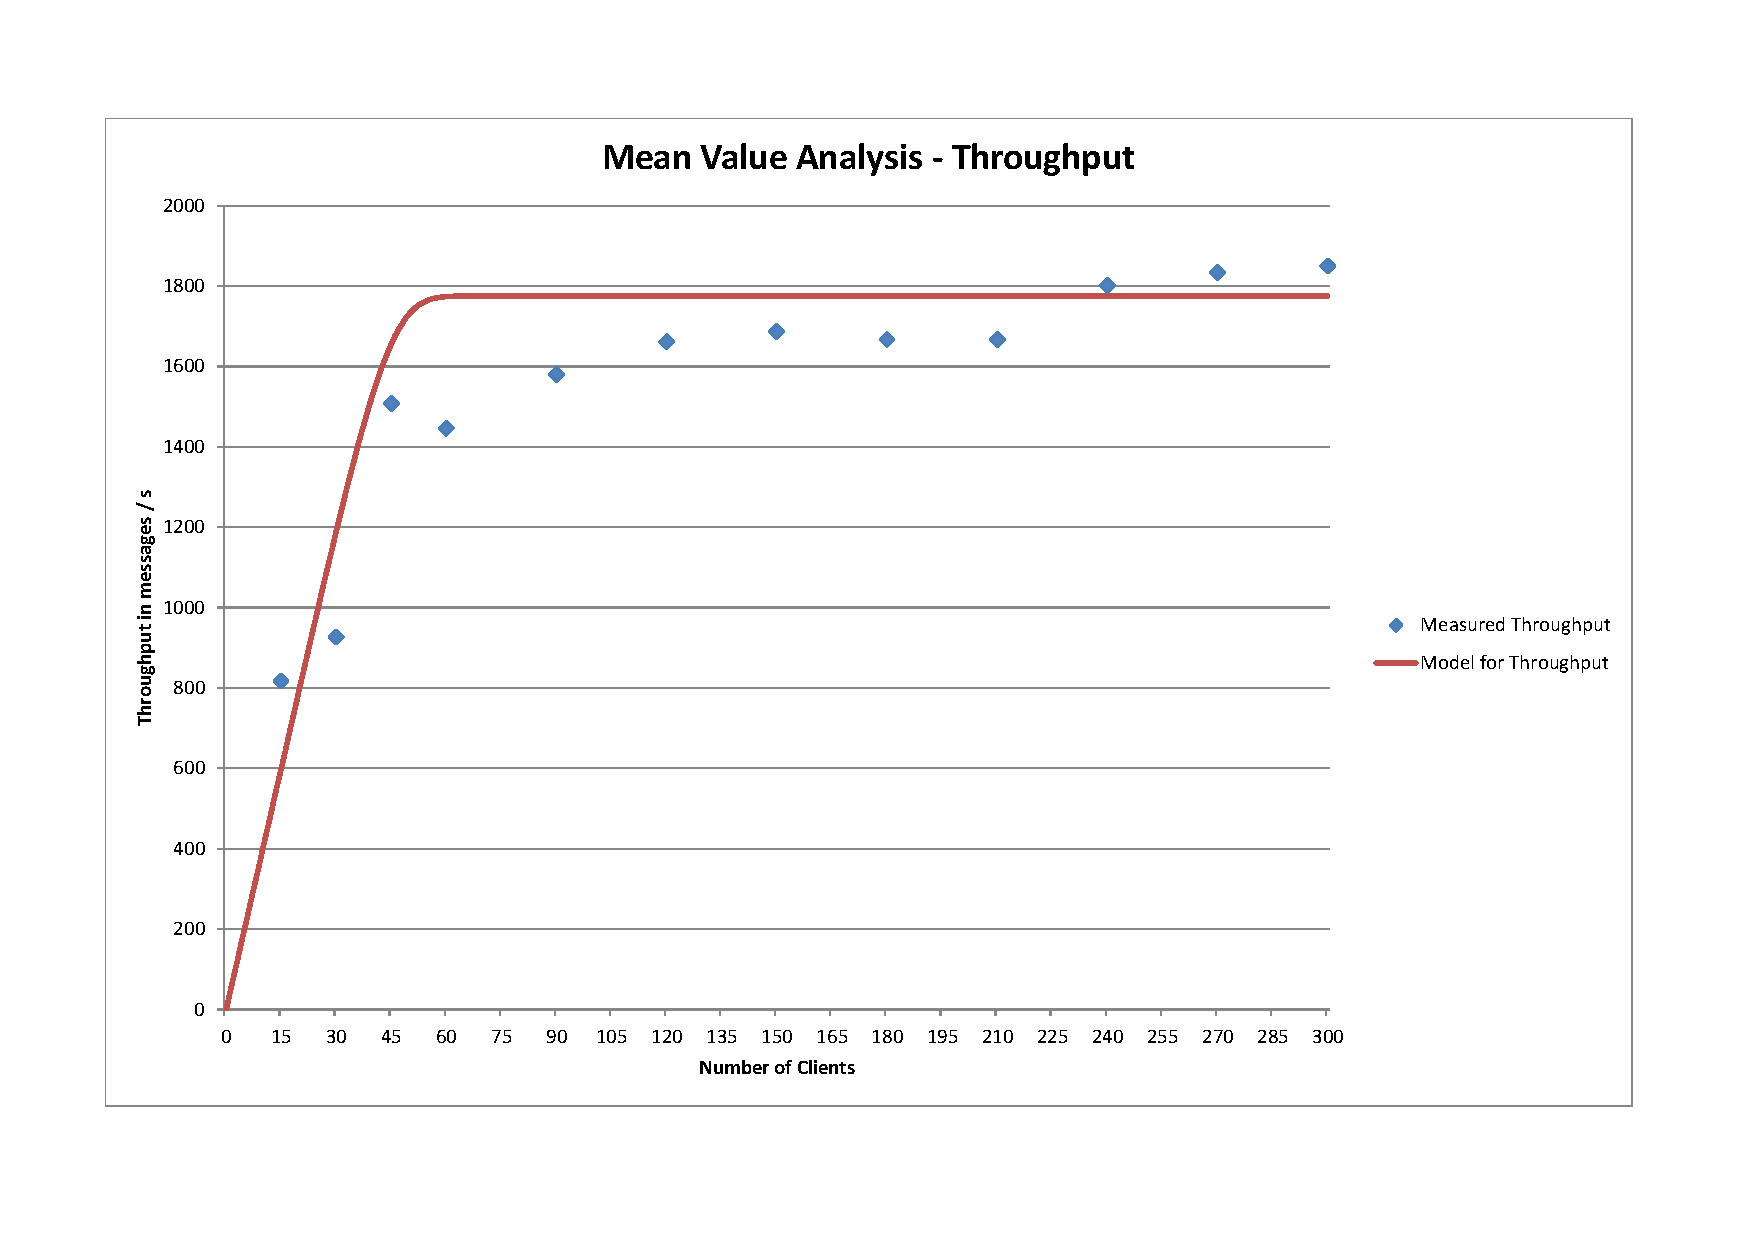
\includegraphics[scale=0.7, trim = 23mm 28mm 24mm 24mm, clip]{measurements_increase_load/tp_total_fixed.pdf}
  \end{center}
  \caption{mean value analysis, throughput fixed}
  \label{fig:tp-total-fixed}
\end{figure}

\end{landscape}



\pagebreak

\section{Measurement Analysis}
\label{sec:measurement-analysis}

Here, the calculated numbers are sanity checked by using the formula $$X_{Throughput}=\frac{N_{Users}}{R_{ResponseTime} + Z_{ThinkTime}}$$ and calculating the following values:

\begin{table}[h!]
\begin{center}
\begin{tabular}{|r|r|r|r|r|r|r|}
\hline
\textbf{N} & \textbf{R[ms]} & \textbf{Z[ms]} & \textbf{$X_{calculated}$[ms]} & \textbf{$X_{measured}$[ms]} & \textbf{Difference[ms]} & \textbf{Difference[\%]} \\ \hline
15  & 10,723 & 10 & 723,814  & 817,027 & -93,212 & -15,546 \\ \hline
30  & 20,179 & 10 & 994,055  & 926,297 & 67,759  & 5,692   \\ \hline
45  & 21,732 & 10 & 1418,136  & 1507,697 & -89,561 & -5,407 \\ \hline
60  & 32,096 & 10 & 1425,316  & 1446,077 & -20,761 & -1,17 \\ \hline
90  & 48,015 & 10 & 1551,315  & 1580,17     & -28,855 & -1,625 \\ \hline
120 & 60,31 & 10 & 1706,73  & 1660,81     & 45,92  & 2,587  \\ \hline
150 & 72,462 & 10 & 1819,013  & 1686,697 & 132,316  & 7,453  \\ \hline
180 & 91,651 & 10 & 1770,771  & 1666,433 & 104,338  & 5,877   \\ \hline
210 & 109,296 & 10 & 1760,33   & 1666,7      & 93,63  & 5,274  \\ \hline
240 & 116,423 & 10 & 1898,383  & 1801,643 & 96,74  & 5,449  \\ \hline
270 & 129,938  & 10 & 1929,42   & 1833,88     & 95,54  & 5,381  \\ \hline
300 & 146,625 & 10 & 1915,402  & 1849,807 & 65,595  & 3,695  \\ \hline
\end{tabular}
\caption{measured throughput compared to calculated throughput}
\label{tab:sanity-check}
\end{center}
\end{table}

In figure \ref{fig:tp-sanity-check-total-fixed} the $X_{calculated}$ is displayed and compared to the measured throughput. The difference in percentage is actually quite small, which can also be seen in the table \ref{tab:sanity-check}.\\

The reason why the throughput is less exact then the response time is that a small deviation in the response time has a big effect when the throughput is calculated, because the measured response time multiplies.\\

\begin{landscape}\begin{figure}[H]
	\begin{center}
    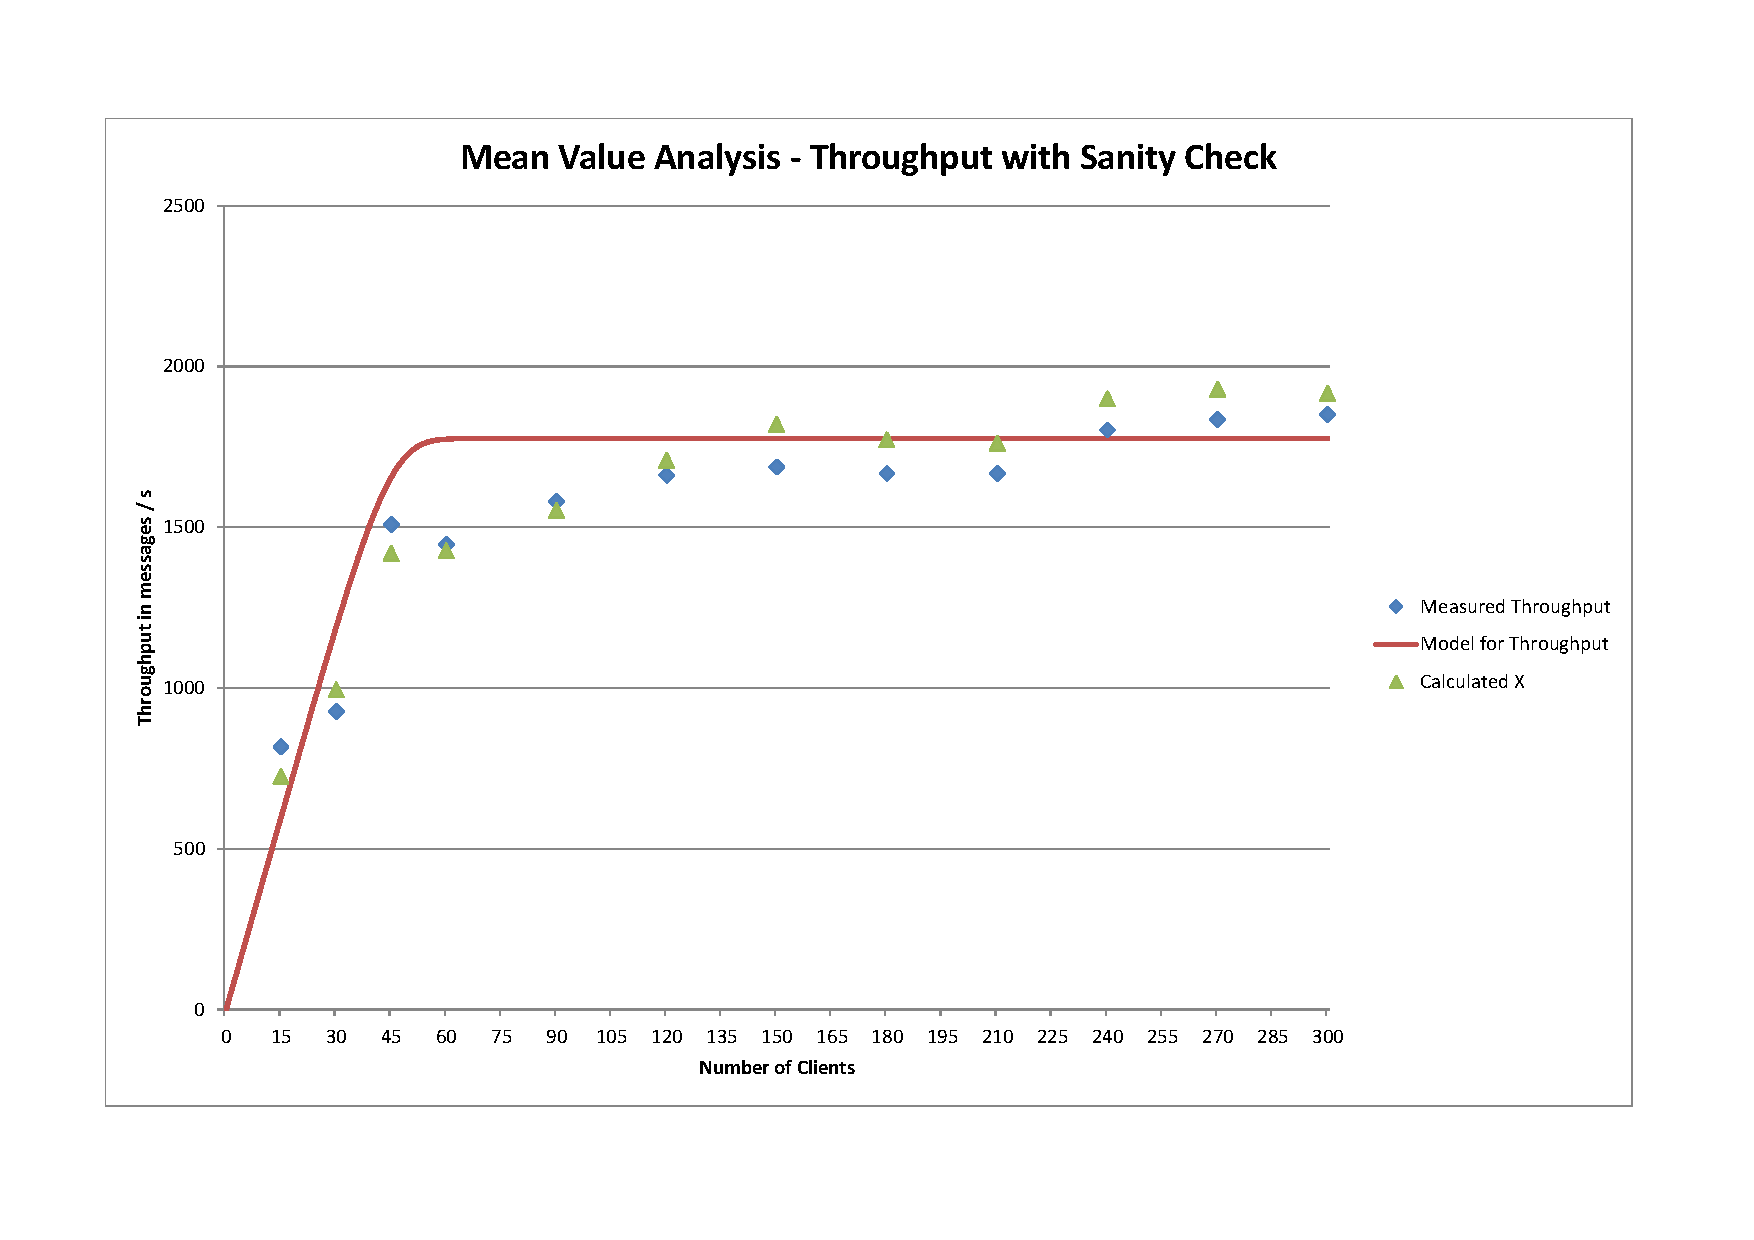
\includegraphics[scale=0.7, trim = 23mm 28mm 24mm 24mm, clip]{measurements_increase_load/tp_sanity_check_total_fixed.pdf}
  \end{center}
  \caption{mean value analysis, throughput fixed, with sanity check}
  \label{fig:tp-sanity-check-total-fixed}
\end{figure}
\end{landscape}


\subsection{Mismatch Explanation Model v.s. Measured Data}

There are several reasons why the model doesn't match the measured data perfectly.\\

Firstly, as already described in the very first chapter, the assumptions to model a queueing network don't hold fully, so there will be deviations.\\

Next, the queueing model is a very simplified version of the real system, so that it's less complicated. The downside of this is that the model of course is not exact.\\

Nevertheless, the model can show global trends of the messaging system. Therefore it can predict how the system might change when implementing things differently. Due to the fact that building, actually implementing and configuring more complex parts of the system (e.g. multiple databases) is time consuming and in practice often a cost factor, models like this can help estimating which components could bring significant performance improvements.\\

\subsubsection{The Bumps}

After doing the analysis, the reason for the ugly bumps in the graphs were discovered: The algorithm to simulate the queuing network works with doubles. This leads to numerical instabilities because it works with very small and very numbers. These instabilities can be avoided when the Java algorithm would be changed to use BigDecimal instead of double. However, for the interpretation of the test results it doesn't matter, because one can easily interpret the model if it wouldn't have those bumps. Unfortunately, there was no time left for implementing this.\\


\pagebreak

\section{Scaling the System}

In this section, the model developed in the previous section is used to simulate what would happen if certain components would be implemented differently, scaled differently, or optimized furthermore. It shows how the model is a powerful tool to consider implementing new features, or even more important, why certain costly features should not be implemented from a performance point of view.\\


\subsection{Database}

The Java program was extended so it can locate the bottleneck component of the system. The reason why the database is listed first here is that the database is the bottleneck of the model. Figure \ref{fig:tp-db-scale} shows that the throughput would grow linearly, as we would expect it. And figure \ref{fig:rt-db-scale} shows that the response time would also grow slower.\\

However, the predicted model seems to be flawed somewhat: While it works well for two database instances, there are some bumps when modelling 3 or 4 databases. Initially, it was assumed that this could have been a possible weak point of this model. However, further investigations showed that the model is fine, but the Java implementation of the queuing network is numerically unstable. To avoid this, a new implementation was created, which used the Java BigDecimal class. Figures \ref{fig:tp-db-scale-stable} and \ref{fig:rt-db-scale-stable} nicely show how the numerically stable version of the Java program creates more accurate results. The downside of the more more precise model implementation is that it is computationally more expensive, but only by a constant factor, compared to the numerically unstable implementation. To be able to do more experiments, I decided to stick with the unstable implementation, so the simulations are faster.\\

To find the limit of the rest of the system and to further validate the model, the database was scaled even more, from 10-30 databaes. However, the one database is displayed too as a reference.\\

To display the database utilization figure \ref{fig:db-utilisation} has been inserted. It is clearly visible that there is a relationship between response time and database utilization. In the real system, this would mean that message start queuing up waiting for the database connection. We also note the bumps which are obviously wrong - it is obviously not possible that the utilisation goes over 100\%.\\

In the figures \ref{fig:tp-db-scale2} and \ref{fig:rt-db-scale2} it shows that the throughput and the response time grow linearly respectively, but only up to 12 databases. Then, another component becomes the system limit. Therefore the models 20 x database and 30 x database overlap exactly and no difference can be distinguished. Again, we also notice the disfigurement / the bump of the model at the peek of the curve. But also again, it is nice to see that the general trend is recorded.\\

If this was a real system, one could decide to invest some work and implement the messaging system with multiple databases. It seems to have a linear effect, which is great in this case. However, there is one caveat which is not captured by the model: There would be additional overhead to either synchornize the databases, or the middlewares would have to connect to multiple databases. This might be insignificant if there are only 2 or 3 additional databases, but it will probably become a concern if 10 or 20 additional databases are implemented. In this case, one should probably refine the model and run the simulations again.\\

\begin{landscape}\begin{figure}[H]
	\begin{center}
    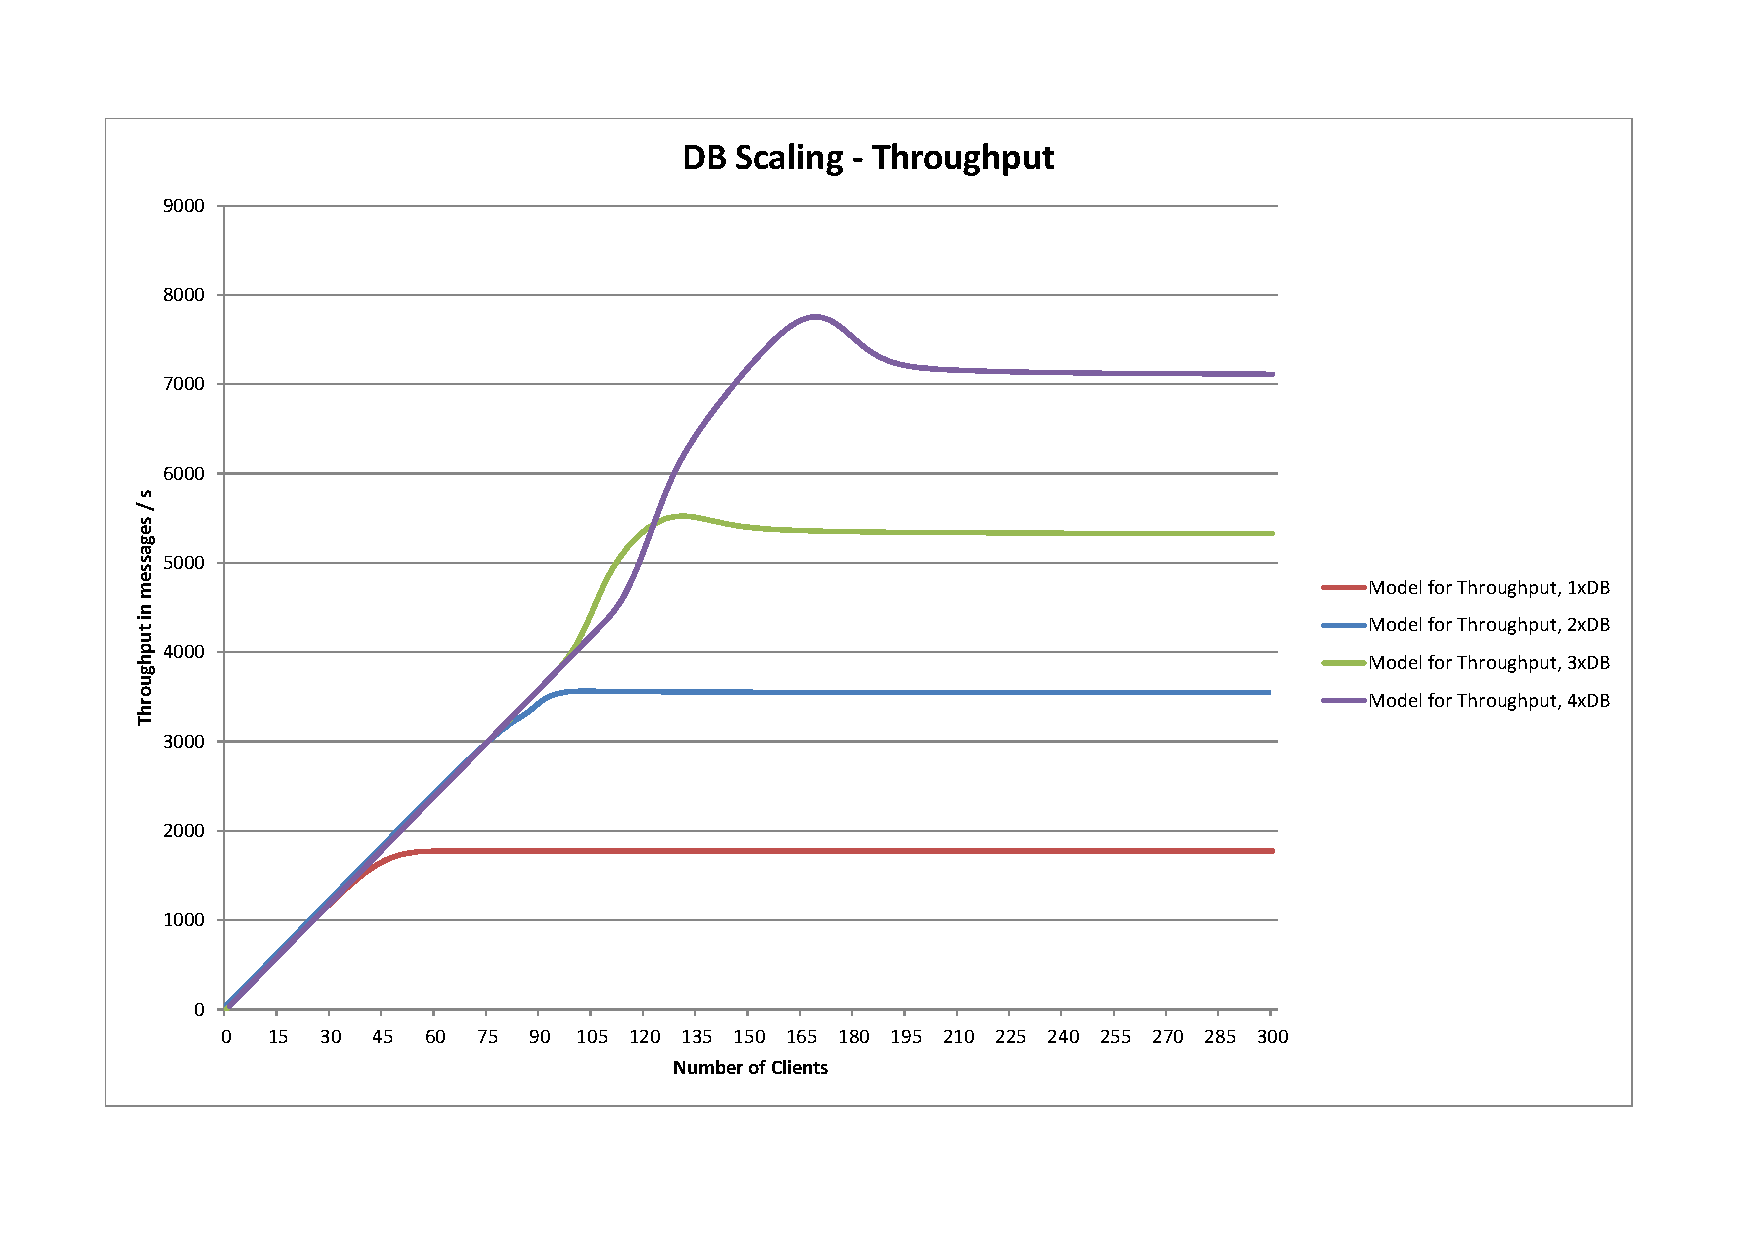
\includegraphics[scale=0.7, trim = 23mm 28mm 24mm 24mm, clip]{measurements_increase_load/tp_db_scale.pdf}
  \end{center}
  \caption{model prediction, throughput database scaling}
  \label{fig:tp-db-scale}
\end{figure}

\begin{figure}[H]
	\begin{center}
    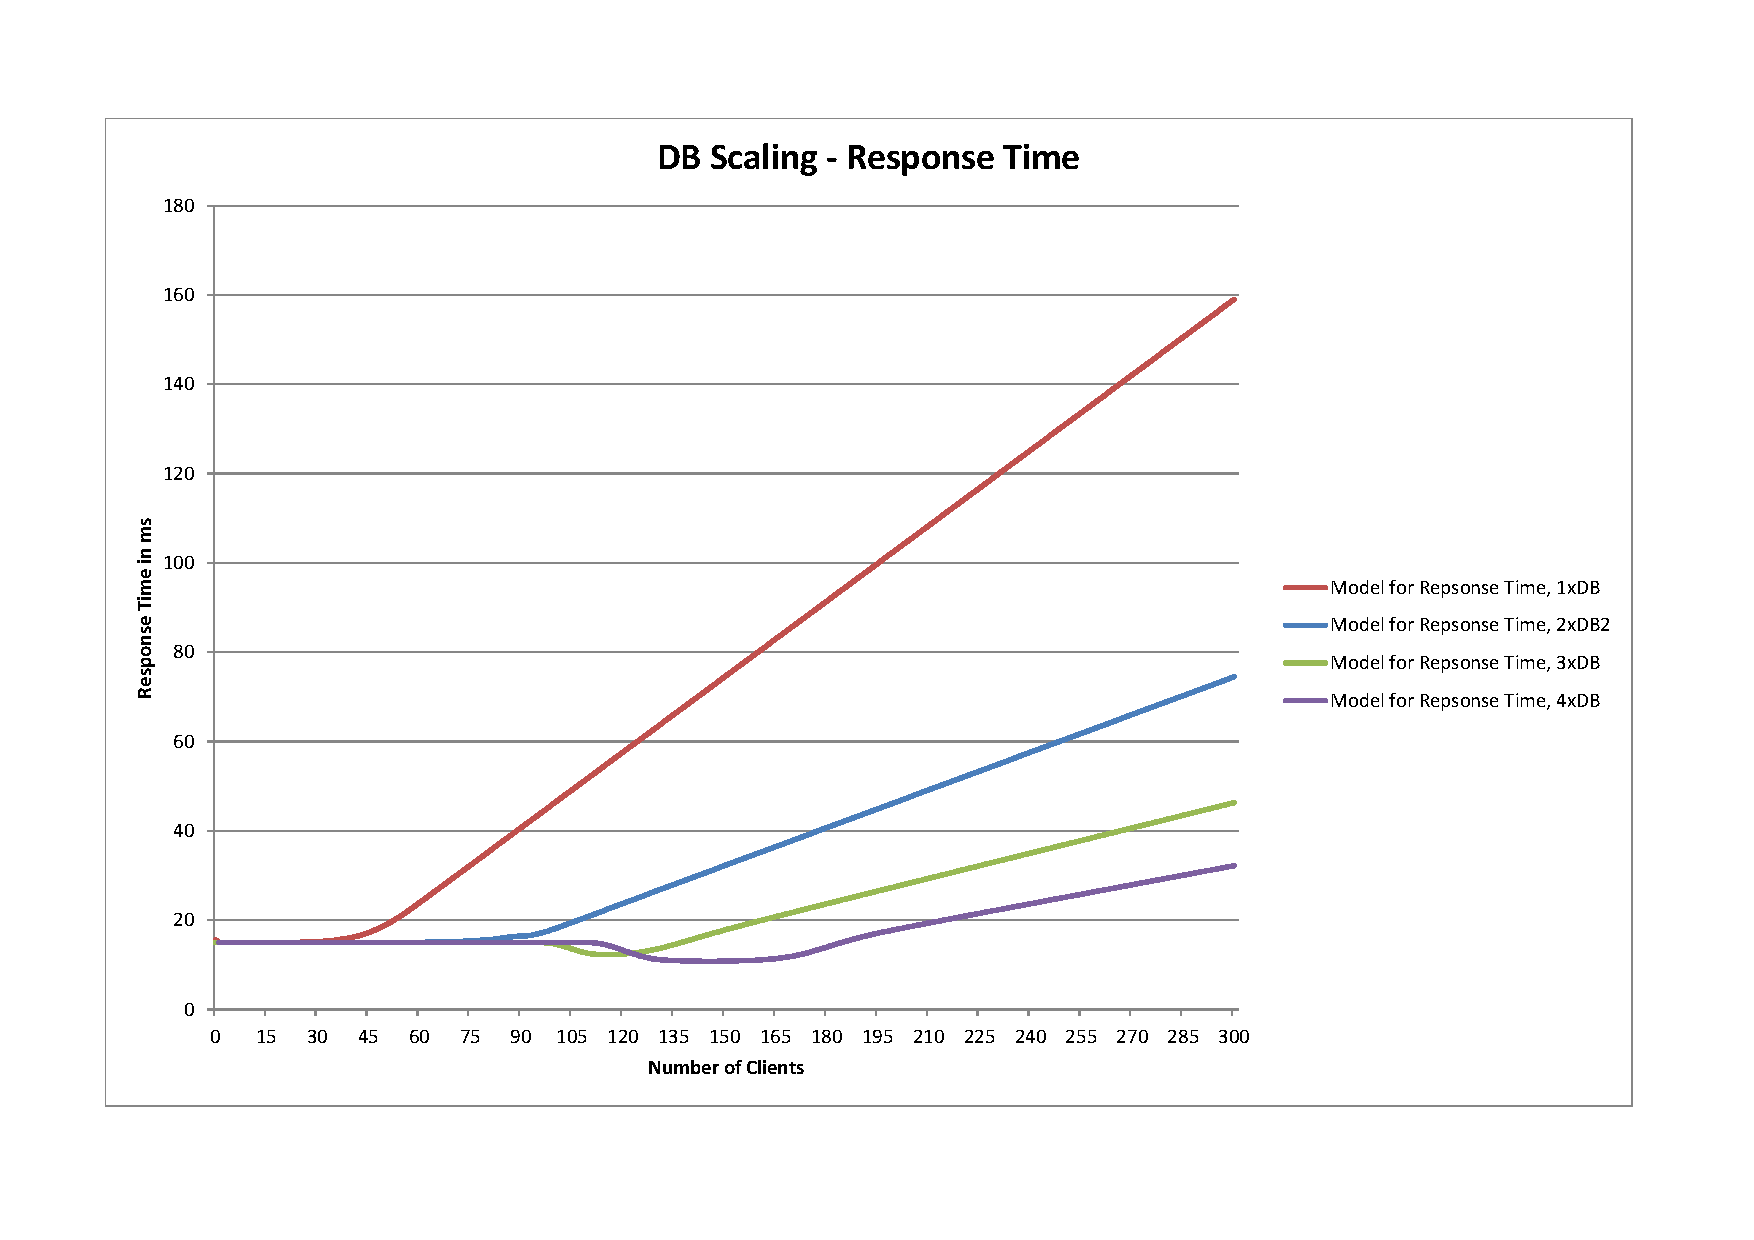
\includegraphics[scale=0.7, trim = 23mm 28mm 24mm 24mm, clip]{measurements_increase_load/rt_db_scale.pdf}
  \end{center}
  \caption{model prediction, response time database scaling}
  \label{fig:rt-db-scale}
\end{figure}

\begin{figure}[H]
	\begin{center}
    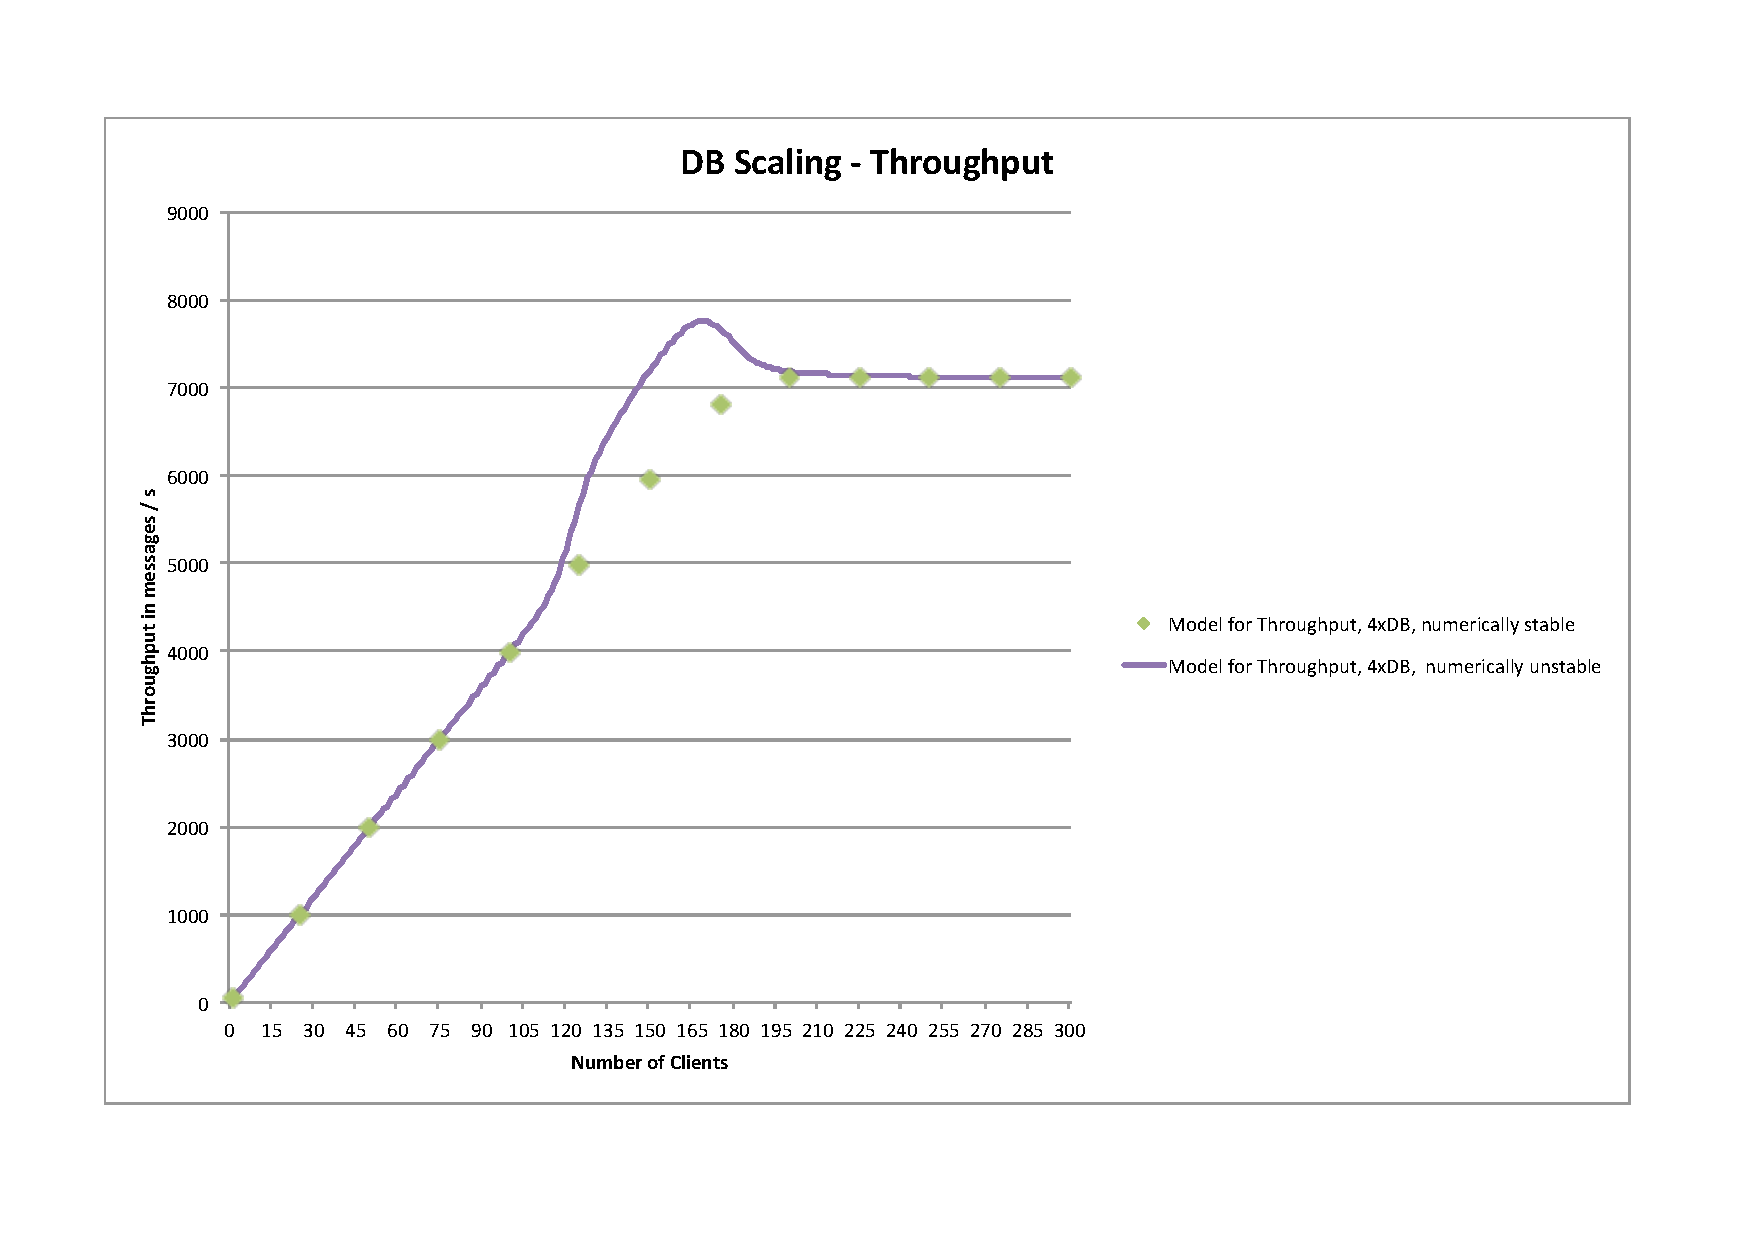
\includegraphics[scale=0.7, trim = 23mm 28mm 24mm 24mm, clip]{measurements_increase_load/tp_db_scaling_stable.pdf}
  \end{center}
  \caption{model prediction, throughput database scaling, stable algorithm vs. unstable algorithm}
  \label{fig:tp-db-scale-stable}
\end{figure}

\begin{figure}[H]
	\begin{center}
    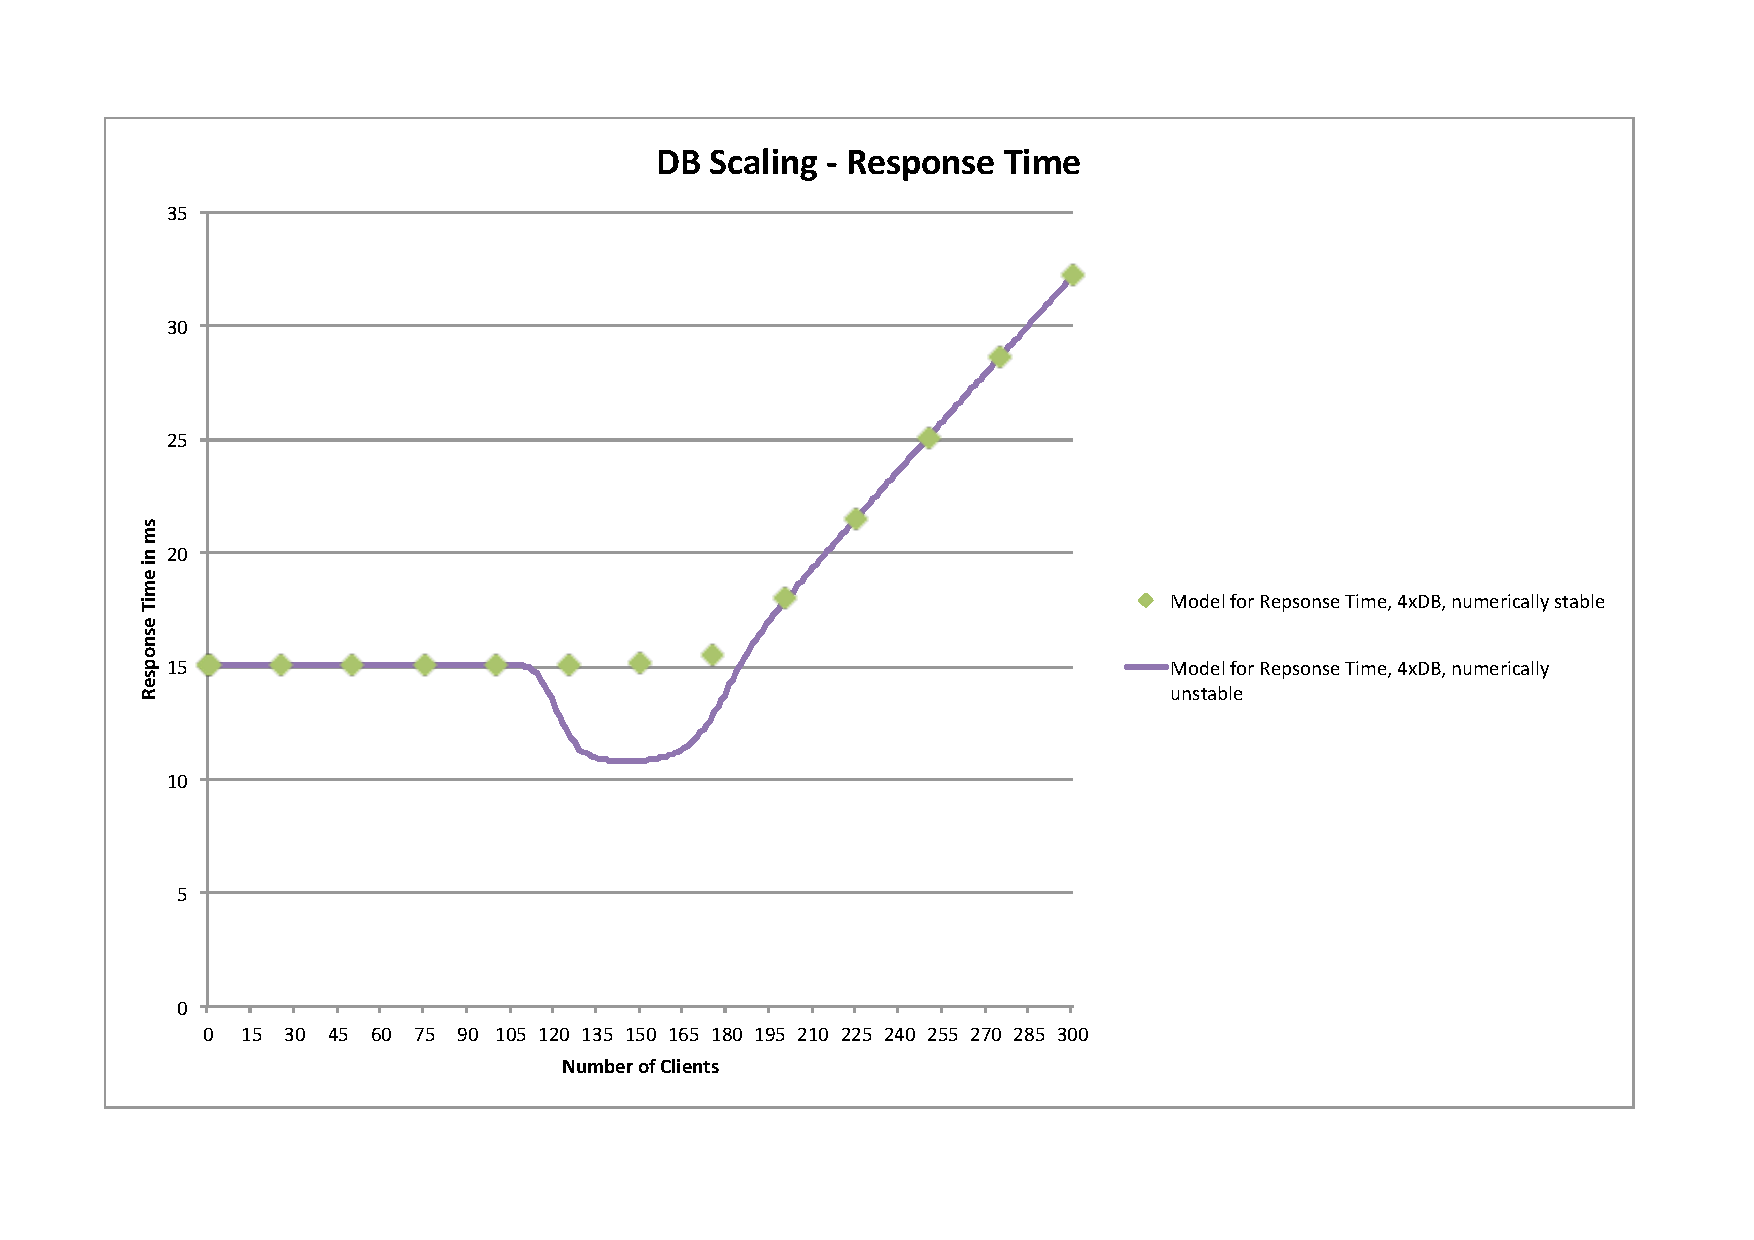
\includegraphics[scale=0.7, trim = 23mm 28mm 24mm 24mm, clip]{measurements_increase_load/rt_db_scaling_stable.pdf}
  \end{center}
  \caption{model prediction, response time database scaling, stable algorithm vs. unstable algorithm}
  \label{fig:rt-db-scale-stable}
\end{figure}

\begin{figure}[H]
	\begin{center}
    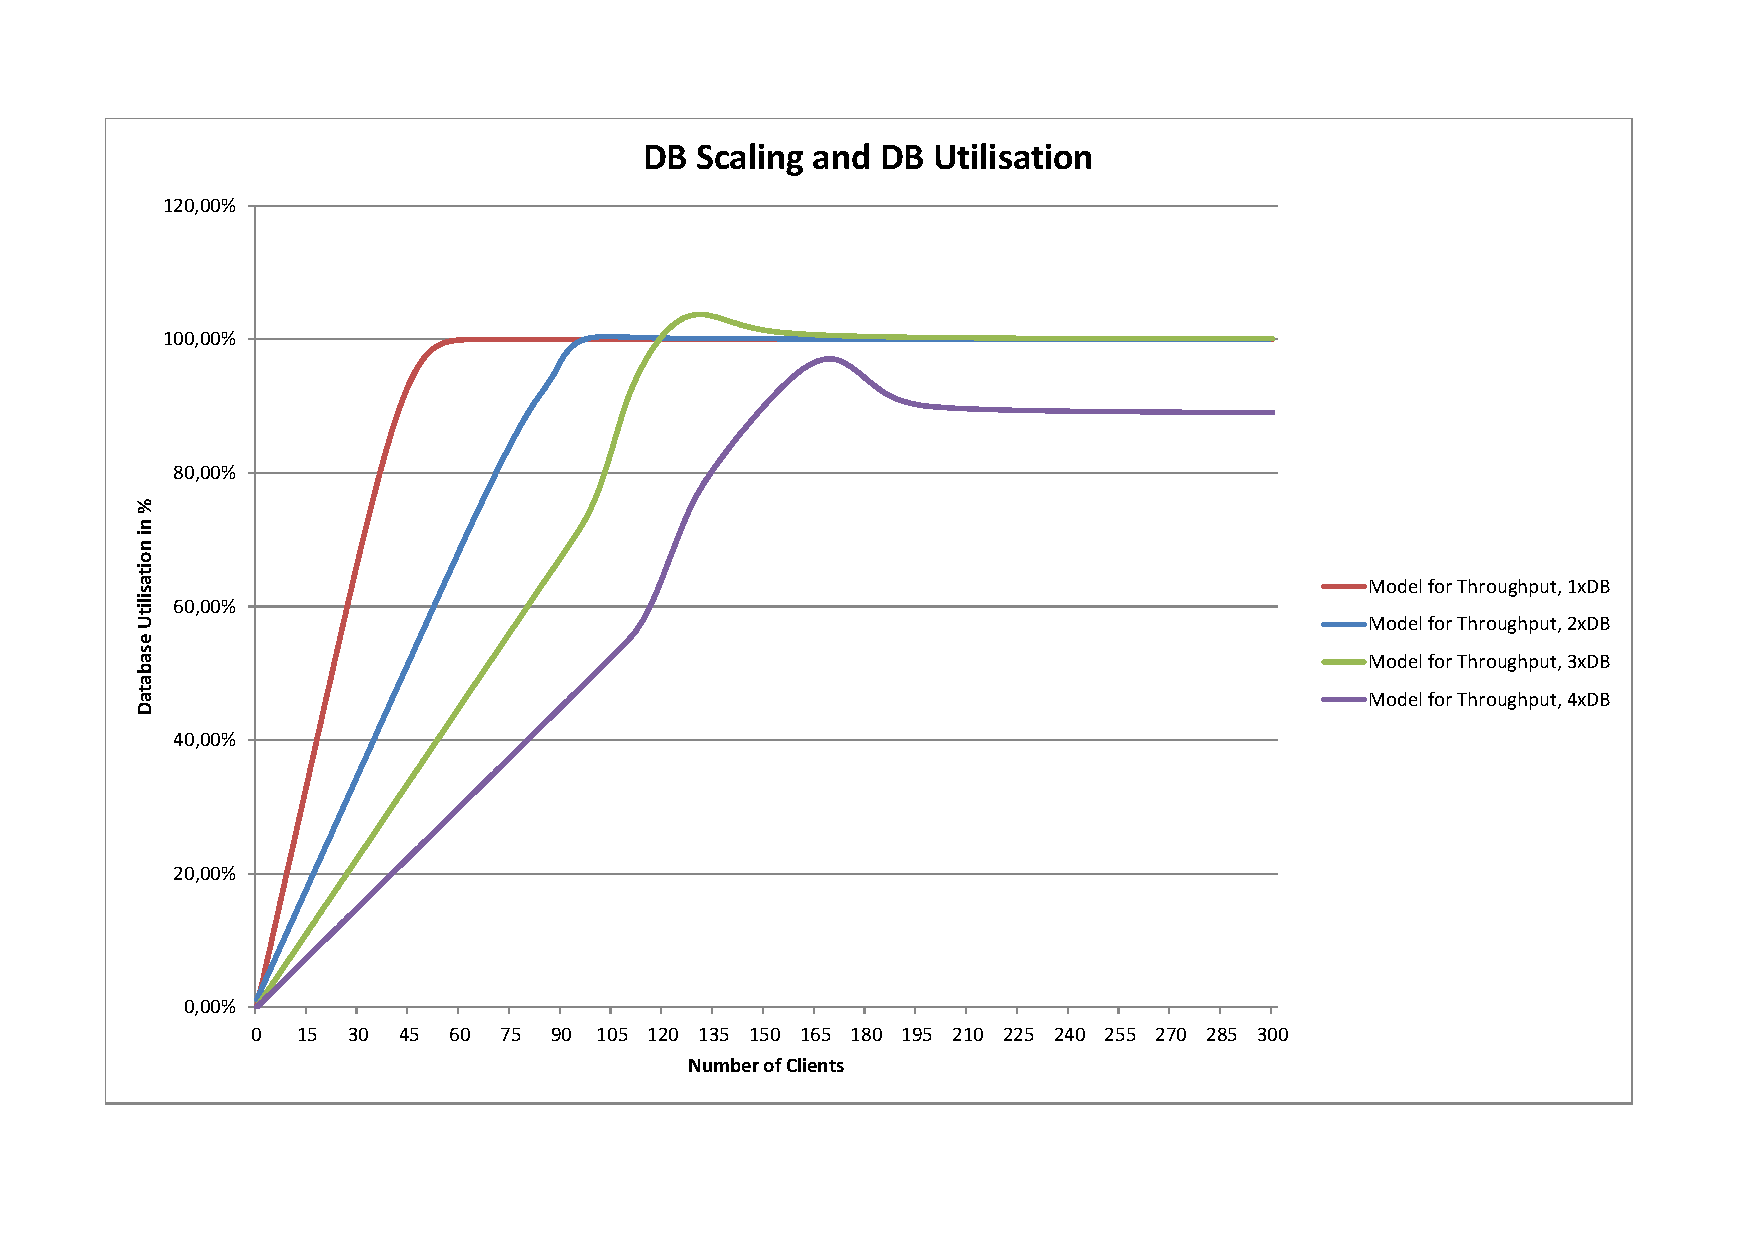
\includegraphics[scale=0.7, trim = 23mm 28mm 24mm 24mm, clip]{measurements_increase_load/db_utilisation.pdf}
  \end{center}
  \caption{model prediction, database utilisation for database scaling}
  \label{fig:db-utilisation}
\end{figure}

\begin{figure}[H]
	\begin{center}
    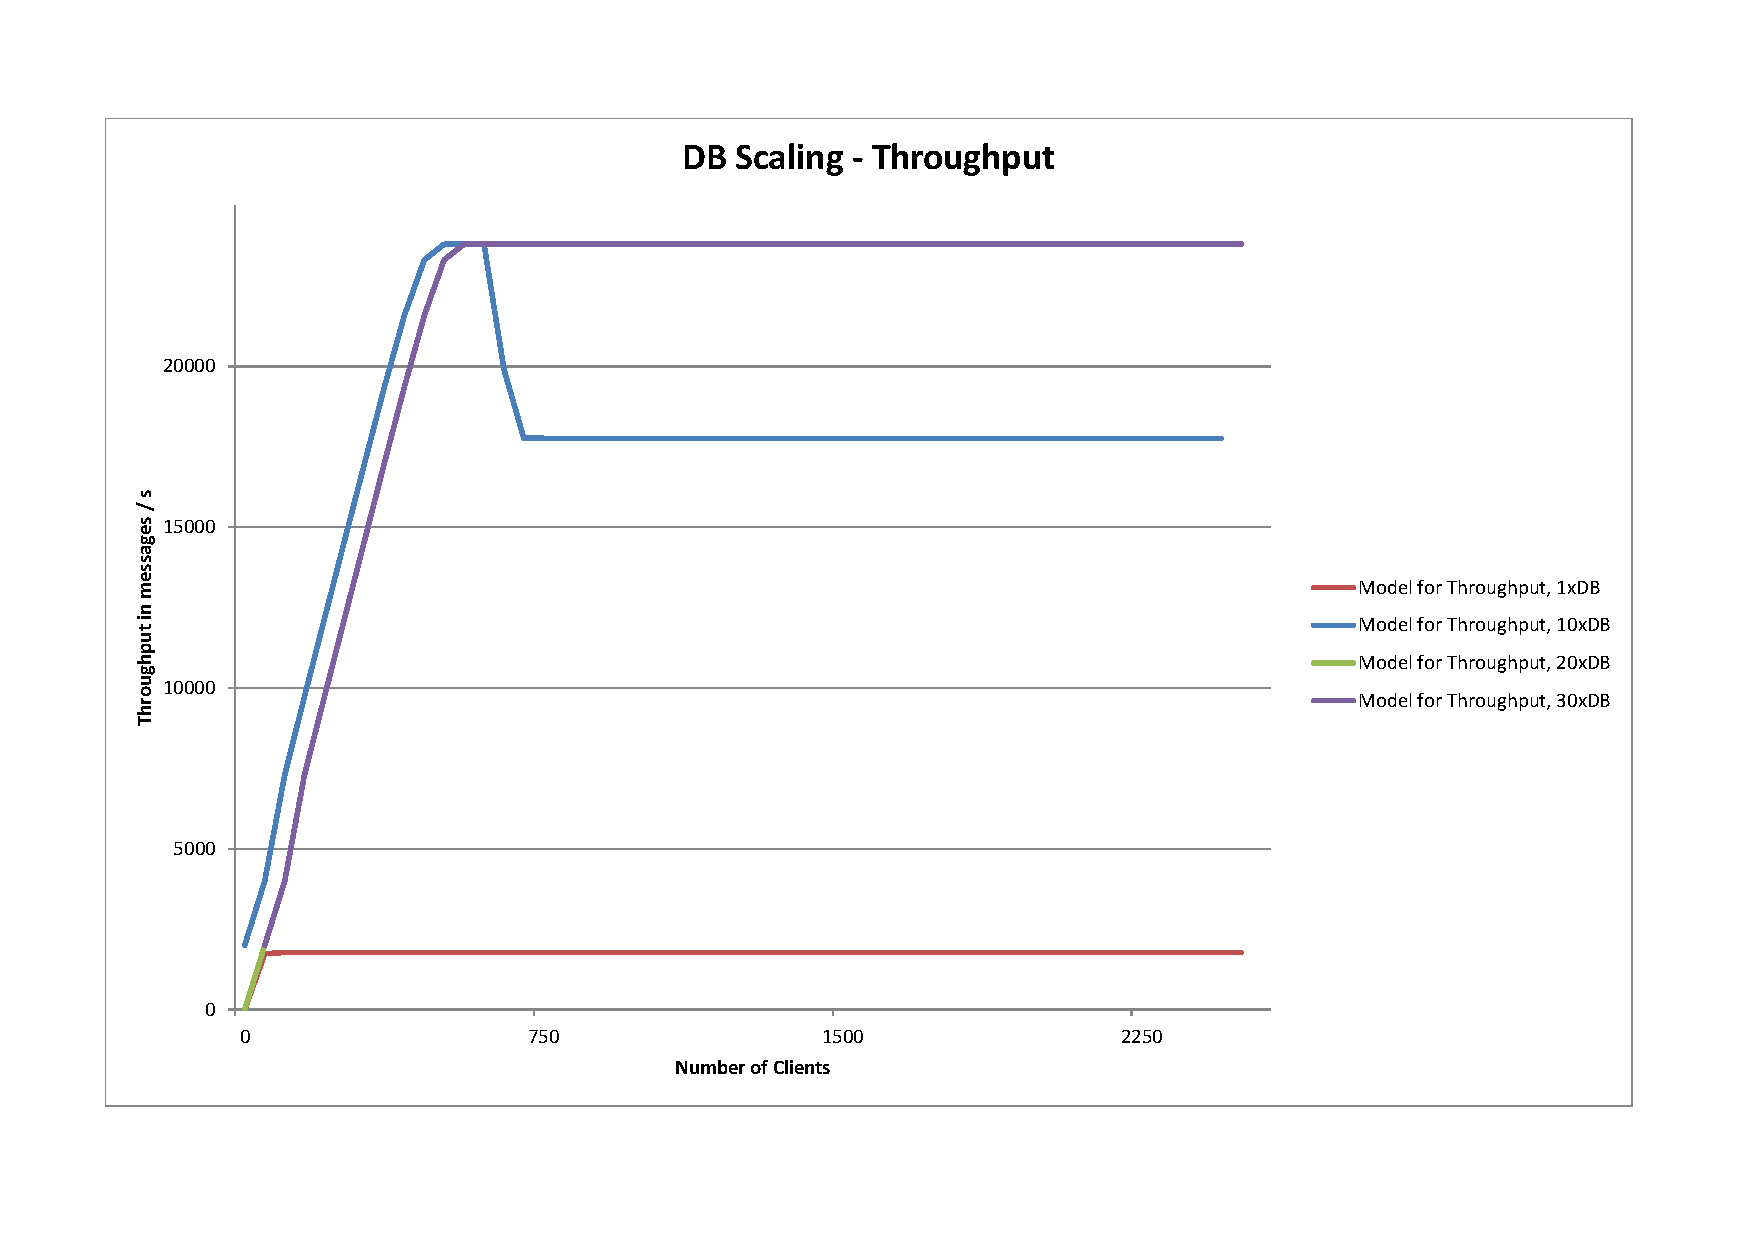
\includegraphics[scale=0.7, trim = 23mm 28mm 24mm 24mm, clip]{measurements_increase_load/tp_db_scale2.pdf}
  \end{center}
  \caption{model prediction, throughput database scaling, high values}
  \label{fig:tp-db-scale2}
\end{figure}

\begin{figure}[H]
	\begin{center}
    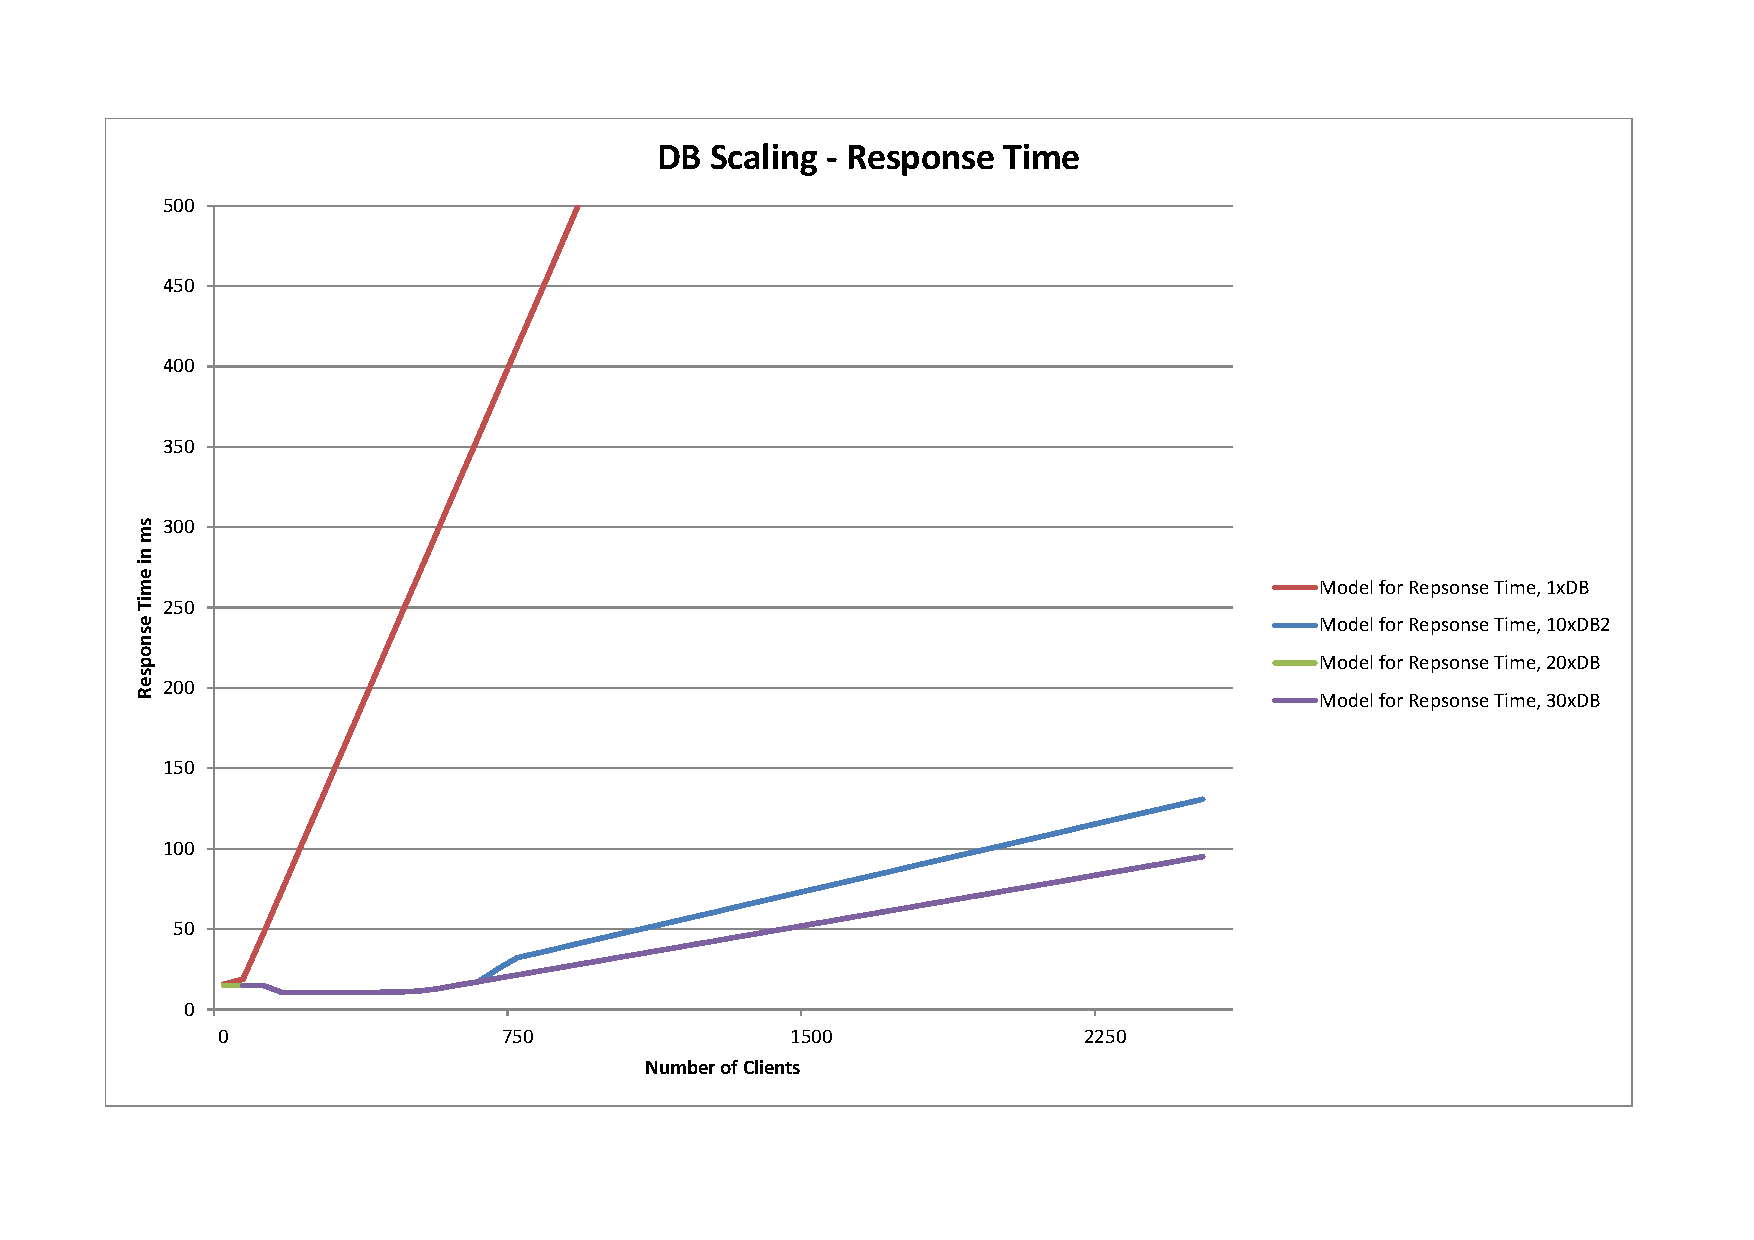
\includegraphics[scale=0.7, trim = 23mm 28mm 24mm 24mm, clip]{measurements_increase_load/rt_db_scale2.pdf}
  \end{center}
  \caption{model prediction, response time database scaling, high values}
  \label{fig:rt-db-scale2}
\end{figure}


\end{landscape}



\subsection{Middleware}

Using this model, the figures \ref{fig:tp-middleware-scale} and \ref{fig:rt-middleware-scale} show that scaling the middleware has practically no effect on the system. This is because one single middleware has a connection pool of 20, which seems to be enough to satisfy about 50-60 clients. Then the requests start queuing at the database level.\\

\begin{landscape}\begin{figure}[H]
	\begin{center}
    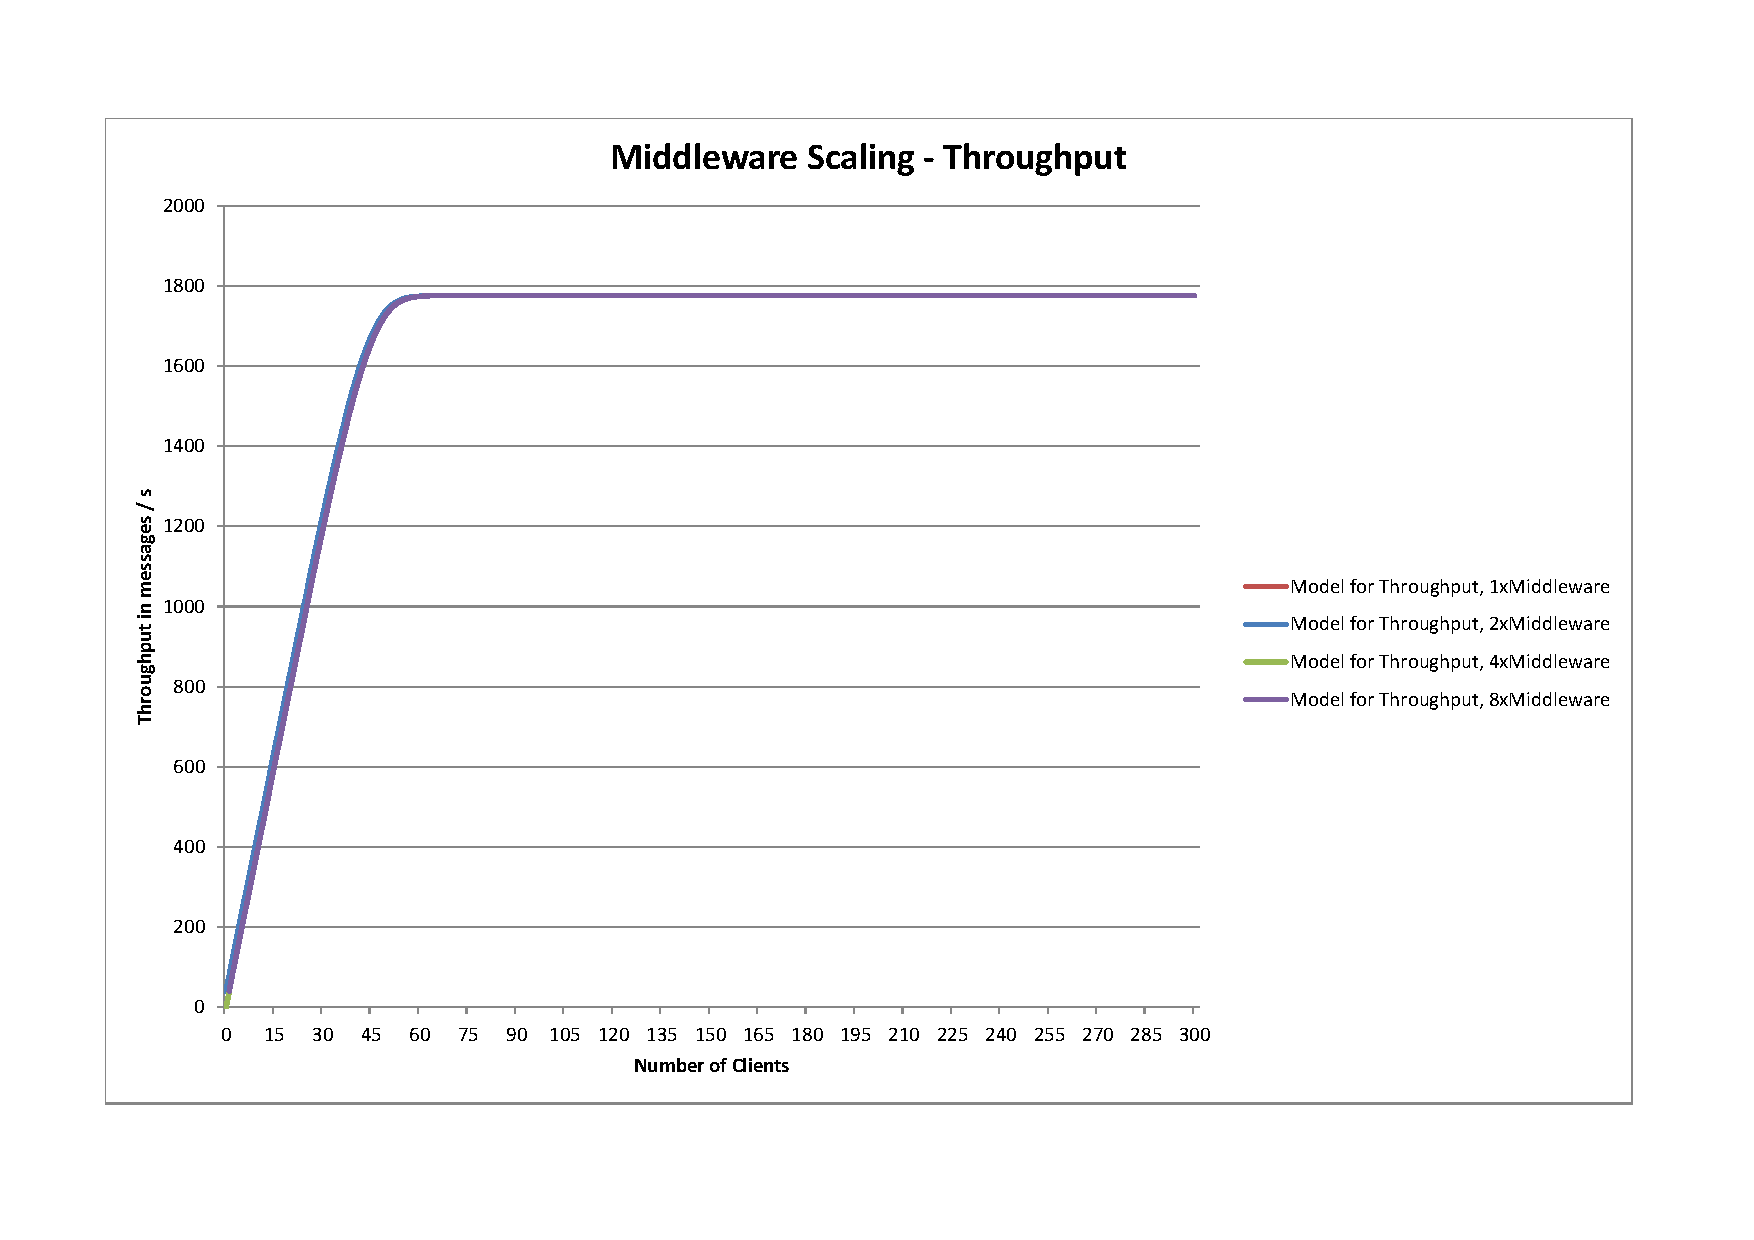
\includegraphics[scale=0.7, trim = 23mm 28mm 24mm 24mm, clip]{measurements_increase_load/tp_middleware_scaling.pdf}
  \end{center}
  \caption{model prediction, throughput middleware scaling}
  \label{fig:tp-middleware-scale}
\end{figure}

\begin{figure}[H]
	\begin{center}
    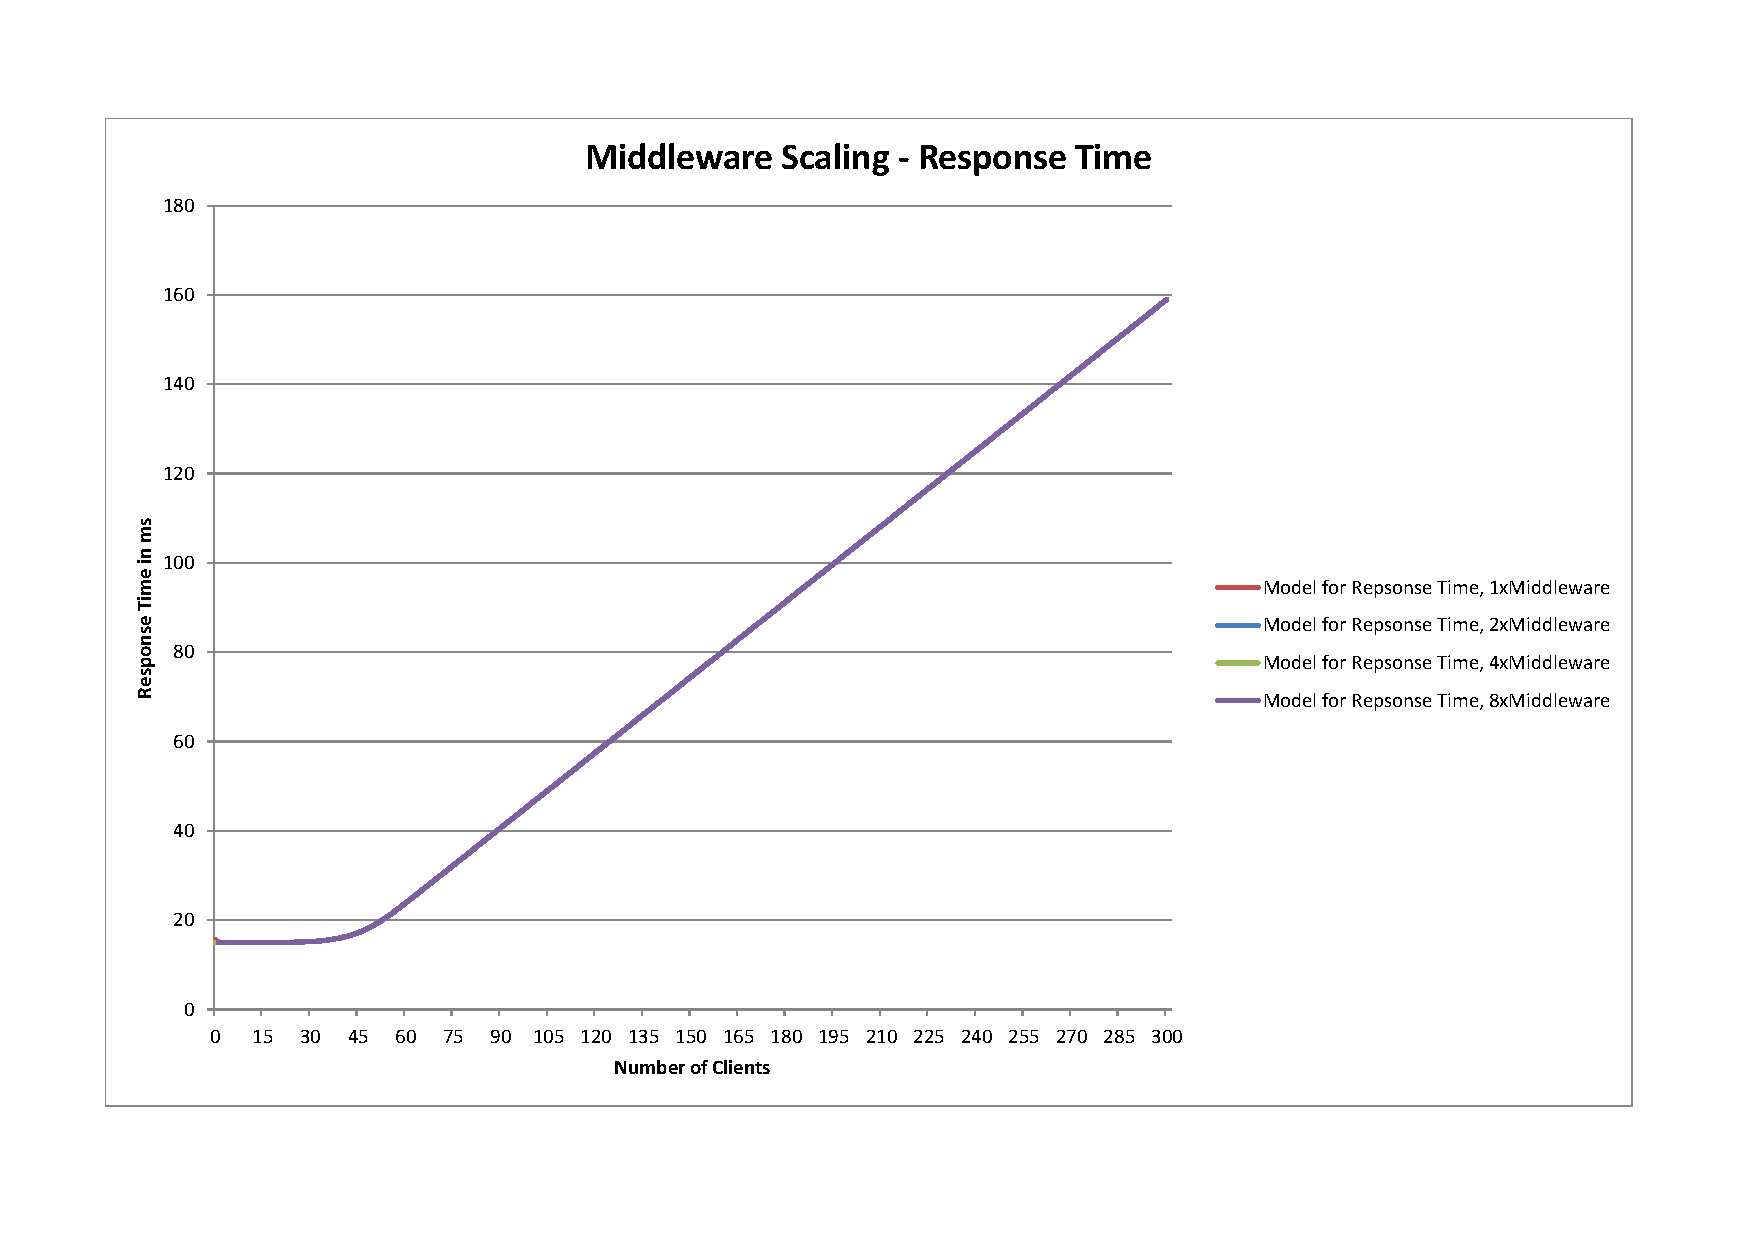
\includegraphics[scale=0.7, trim = 23mm 28mm 24mm 24mm, clip]{measurements_increase_load/rt_middleware_scaling.pdf}
  \end{center}
  \caption{model prediction, response time middleware scaling}
  \label{fig:rt-middleware-scale}
\end{figure}

\end{landscape}



\pagebreak

\section{Conclusion}

First, the assumptions, on which the whole analysis bases on, were stated. There it was already clear that a queueing model would not be an exact solution, but could only be used for rough approximations because the assumptions are not fully met when the system is runnning on the Amazon elastic compute cloud.\\

In this document, the system implemented in the prior milestone\cite{milestone1} is explained by an analytical queuing model. Each component of the system has been modelled individually, and then those components were combined to a queueing network to model the system as a whole. The parameters and how they were obtained is clearly stated, and thus the experiments should be reproducible.\\

Next, the performance characteristics of the model were compared to the measurements obtained in milestone I\cite{milestone1} and during this milestone (scaleout experiments) using the operational laws. In the beginning, it was hard to find a model that fits to the system, but once the first mean value analysis was created, it was then simpler to go to more complex models that fit better to the system.\\

It then was explained where the model and the data match and where they diverge. Extensive explanations were given concerning the code, system and hardware of the system.\\

Finally, the model was used to predict how the system would behave when scaled. This was done using graphs to plot how they would scale. It seems that the system is clearly limited by the database. Scaling the middlewares on the other hand would not have a noticeable effect.\\


\pagebreak

\section{Lessons Learned}

The modelled system seems to predict the behaviour of the system quite well. Unfortunately I believe that some of the measurements obtained in milestone I\cite{milestone1}, especially the microbenchmarks, are not 100\% accurate. Therefore the middleware service time might be a little too low and thus, scaling the middlewares doesn't have an effect on the system as a whole.\\

Even tough there are Tools to analyze queuing systems, like the Java Modeling Tools\footnote{http://jmt.sourceforge.net/}, these tools often are difficult to use and / or are out of date. For example, the Java Modeling Tools did not even run under MacOS, but worked under Windows. It is unclear to me why there is no more sophisticated software, which is easy to use, and up to date, in which a queuing network can easily be simulated with numerical stability.\\

Instead, a Java program was implemented, which obviously is numerically not stable when using big numbers (e.g. for components, or for clients). Even tough the program was fixed, see figure  TODO XXXXXXXXXXXXXXXXXXXXXXXXXXXXXXXXXXXXXXXXXXXXXXXXXXXXXXXXXXXXXXXXXXXXXXXXXXXXXXXXXXXXX
, the performance of the computation for the model decreased dramatically by using BigDecimal instead of double. However, if a real system should be evaluated, then the fixed program can be used, and a long computation would still be preferred compared to implementing the real system and running some tests. For the overview, the fast but numerically unstable variant is a good starting point.\\

However, the power of having a system model cannot be underestimated. Using the system model, one can easily check, whether it is cost and time efficient to invest into system development of certain parts of the system. Especially when it is not possible to build up an infrastructure (e.g. if you want to implement a new network protocol which should be used across the whole internet), such system models play a crucial role in software development and system development.\\

\begin{figure}[H]
	\begin{center}
    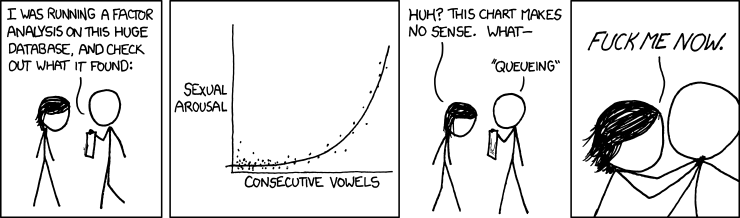
\includegraphics[scale=0.52]{consecutive_vowels.png}
  \end{center}
  \caption{an xkcd comic which relates to queuing theory. Sometimes, you need something to laugh about when correcting these ASL reports. Source: http://xkcd.com/853/}
\end{figure}

\pagebreak

\section{References}



\bibliographystyle{plain}
\bibliography{literature}











\end{document}









